% This example An LaTeX document showing how to use the l3proj class to
% write your report. Use pdflatex and bibtex to process the file, creating 
% a PDF file as output (there is no need to use dvips when using pdflatex).

% Modified 



\documentclass{l3proj}
\usepackage{subfig}
\usepackage{graphicx}

\begin{document}

\title{QPQ Simulation Game}

\author{Almohannad Albastaki \\
        Ronaldas Gadzimugometovas \\
        Tom Gough \\
         Conor McHarg \\
        Borislav Hristov}

\date{31 March 2017}

\maketitle

\begin{abstract}

Team B was tasked to design a financial analysis tool for Adam Smith Business School as part of the Team Design Project. The application was required to facilitate data input and automate data analysis. With utilising extensive planning techniques, such as drawing a UML Class diagram and different levels of wireframes, the team arrived at a decision, among other things, to use Java and JavaFX as programming tools for the project. Team progress was guided by professional software development practices, such as Gitlab continuous integration, and elaborate testing strategy. The lack of team members' experience in professional development world did prove to be a hindrance but ultimately, individual learning and commitment helped to deliver a fully functioning product. As requested by the customer, the final design minimised user effort, encapsulated all game data, introduced import/export functionality and provided tremendous game customisability. Consequently, the product received positive client feedback yet it was acknowledged that there was room for additional features.

\end{abstract}

%% Comment out this line if you do not wish to give consent for your
%% work to be distributed in electronic format.
\educationalconsent

\newpage

%==============================================================================
\section{Introduction}
\label{sec:introduction}

This document presents the dissertation of Team B, a team consisting of three third year Electronic and Software Engineering and two Mobile Software Engineering students, financial analysis tool. The tool was developed for the Adam Smith Business School (ASBS) to act as a financial aid for their Quid Pro Quo (QPQ) simulation game. The primary aim of the tool was to provide an efficient and simple manner of processing, storing, and exporting the output from the simulation game.

The document delves into software development processes practised by Team B throughout the project and how these practices affected the team's decision-making, planning, and development techniques. Through this case study, Team B aims to achieve a better understanding of why these processes were taught in the Professional Software Development course at the University Of Glasgow, and how to better implement them in a future team, or individual, projects.

The QPQ game itself is a hands-on paper-based simulation game which mirrors a typical production line found in most modern organisations. Participants of focus are usually second-year business students. Students are required to complete "orders", with appropriate timeliness, to see a profit. When the game comes to a halt a financial analysis from the resultant data is conducted. The main goal of the simulation game is to teach these Business students the importance of employing various business process theories, and how these processes affect any given production based organisation.  

The dissertation is structured as follows:

Section \ref{sec:casestudy} - Case Study Background - outlines the case study in more depth. Details of the customer, preliminary objectives, stakeholders, team aims, initial team planning, and the final product are further discussed in this section. This section also mentions the workings of the game, as interpreted by the team, and the key solution to the issue faced while playing.

Section \ref{sec:teamdynamics} -  Team Dynamics - details the team composition and dynamic. The team had opted for a laissez-faire styled leadership structure, where each member has equal decision power. The benefits/consequences of this and how it affected the development process are reflected upon throughout this section.

Section \ref{sec:planning} - Planning - various planning techniques, such as wireframes and class diagrams, were employed throughout the project and their effects are discussed further. The section also discusses project management means, namely Gitlab and its features.

Section \ref{sec:meetings} - Meetings - discusses the purpose and the outcomes of group and client meetings and outlines the benefits.

Section \ref{sec:communication} - Communication - describes the means of communication both within the team and with the customer and discusses key difficulties.

Section \ref{sec:testing} - Testing - an elaborate three step testing strategy was employed to test the program and ensure all its features perform correctly and return valid results.

Section \ref{sec:development} - Code Development - elaborates on the front-end and back-end development. This section involves a discussion with regards to the technology choices made and the effects these decisions had on the project. The greatest challenge here was the learning curve involved in the technology used and trying to implement the required functionality.

Section \ref{sec:finalproduct} - Final Product Features - summarizes the state of the final product, outlining its features in the light of the of the initial customer requirements.

%==============================================================================
\section{Case Study Background}
\label{sec:casestudy}

\subsection{Customer}

The Adam Smith Business School, a professional research institution committed to the field of business and economics, situated at the University Of Glasgow, had developed a QPQ simulation game, to be utilised during business tutorials to give students a hands-on experience of the workings of the production line, to ultimately supply a customer with the required demand.

The QPQ simulation game is the brainchild of Dr. Rob Dekkers, a Reader in Industrial Management at the ASBS, and his team of PhD research students. Dr. Dekkers has written publications on the concepts of Bottlenecks, Engineering Processes, and Production Management. The solution to the simulation game consists of following a number of business process theories from these focuses.

Throughout the project our main point of contact was Dr. Rob Dekkers himself, however often accompanied by his research students; Maria Koukou, Mohammed Aldossary, and Qijun Zhou; All of whom often provided useful information of business theories during the meetings.

\subsection{Preliminary Objective and Stakeholders}
The research students of Dr. Dekkers, not able to attend himself, had conducted the first introduction of the game and issues they faced. The QPQ simulation game is a paper based game which reflects a real life production line. The idea behind the game is that a certain amount of orders for cars (lego cars in the simulation game) are made by a game leader, usually a PhD student. These orders, which currently are comprised of multiple sheets of paper, are passed between students (employees), who act in accordance to their assigned departments (e.g. Production Planning, Good Receipt, Sales) all controlled by a hands-off manager, who is a student him/herself. 

The game consists of three 20 minute rounds in which employees must complete all orders within a time scale to see a profit. The manager, and fellow employees, are given the opportunity to discuss solutions, various practices, and even rearrange themselves to achieve the desired profit at the end of each round. External AYN (As You Need) employees can be hired to assist employees in their respective departments before and during rounds. The AYN employees in most tutorials conducted are PhD students, who have the expertise and knowledge behind the game.

At the end of each round, a financial report is produced. This was stressed to be a very cumbersome effort as it involved looking through many forms, previously filled in by employees, and producing calculations from the variables gathered. The financial department is usually a collective effort of a student, the manager, and a PhD student, to assist. After each round, the financial department would be required to look through the multiple orders produced and calculate a revenue and various, specific, expenditure figures to calculate the profit/loss seen in that round. On average the financial department would be faced with about 20 (or more) filled in forms. Due to this activity, the game sees many delays and students are often left waiting 15-20 minutes between rounds.

The whole game would last around 2 hours, which to Dr. Dekkers was not a satisfactory run time for only 3 rounds. As a result of the wasted time of the financial stage, tutors are forced to reveal the solution in a quick, sometimes unclear, manner. In his view, the students, who were seen as the main stakeholders for the project, must be given more time within the rounds to be able to solve its workings themselves. This meant striving for a greater amount of rounds per tutorial, and secondarily, providing means for keeping figures and variables coherently documented for later study by all users of the game.

The solution to the game involves employing Enterprise Resource Planning (ERP) and discovering bottleneck within the production line to properly see a profit. A bottleneck is defined as a point where activities slowdown due to a department not coping with the coming workload. In further detail, the source of the problem is the lack of building components at the production phase, this is the location of the bottleneck. By recognising this bottleneck and employing ERP, employees will be required to supply the production department in a just in case manner, where common building components are supplied before an order for a car consisting of this component is made, to see an overall profit for the round.

\subsection{Aims}
Dr. Dekkers and his team had taken the stance of allowing the developers to use their creativity to developing the product's functionality as per the initial introduction and a game demonstration provided. With regards to the issues mentioned on the financial analysis, it was seen that reducing this time was key. The main challenge here was translating human processes into a computation and furthermore visualising this in a readable and coherent manner. It was however stressed that an export functionality was to be produced out of these computations, which essentially meant data storage and file writing capabilities.
    
It was as well mentioned that there was no guarantee of a network connection during some tutorials and due to the various computer and smartphone platforms used by students and tutors; a consensus was made that a cross-computer platform application was to be developed. This meant developing using a single language that was able to execute itself on any platform.
Ergo, to define the primary aim, it was decided upon that a computer application to mimic the financial department's forms/activities would best deal with the game's timing and documentation issues without interfering too much with the hands-on experience it currently provides.

\subsection{Project Scope}
 Through many discussions the decision was taken to develop a localised application that could be run on one laptop and would focus on one of the most time consuming aspects of the game, the financial analysis. The customer much preferred this plan to a digitisation of the game as it provided them with an improvement to the game without making it reliant on technology. While the team was happy to develop a wi-fi reliant high end game, in this case the team had to align their objectives with the customer's. The decision the team made on the project scope was taken after several discussions with the customer in which multiple different proposals were put forward until the team settled on an idea the customer was happy with and that they felt would fulfil their requirements.

%==============================================================================
\section{Team Dynamics}
\label{sec:teamdynamics}

The project brought together two Mobile Software Engineering and three Electronics and Software Engineering students. Each participant proved to have specific skills, relevant to the project and preferences, in terms of tasks and the project as a whole. The differences in terms of the study programs did not prove to be a factor.
 
When it comes to organisation, team members had equal decision-making power. The team chose to avoid hierarchy within as no member had considerably more expertise than the others. On the other hand, individual members would step up when feeling that their contribution was valuable and step down when the others seemed more knowledgeable. 

Even though the team was well balanced and had little if any problems working together, there were a few things that hindered the effectiveness of the team. First, each team member had their own personal goals, preferences, and biases which were given priority over the project at some stage or another. For example, in the beginning of the course, the team was more eager to push their own ideas and design goals to the customer than designing in response to customer needs. However, due to continuous progress self-evaluation, the team noticed the lack of effectiveness and measures were taken to avoid this, namely documenting precise requirements and ticking them off once addressed. 

A similar issue was that each member had different coding styles and experience. For example, preferred coding strategies, choice of data types, code readability, etc. caused the team to be inefficient. Team coding process involved the members working on different parts of the program separately first and then the group would integrate the work. Unfortunately, given the differences mentioned above, large portions of good working code needed to be modified or completely replaced in order to make all integral parts compatible with each other. 

Naturally, the team took the time to consider possible ways of minimising the effect of team differences in further development. One of the strategies included careful allocation of tasks which would minimise integration effort. Furthermore, the team agreed to put additional effort foreseeing potential integration issues (e.g. variable naming) and preparing themselves (e.g. agreeing on the shared variable names in advance).

%==============================================================================
\section{Planning}
\label{sec:planning}

\subsection{Initial Planning}
Initial requirements gathering involved a full demonstration of the game. It was here that team members got themselves involved directly in the game, with the assistance of Adam Smith Business School students and another PSD 3 team. Each team member was to keep note of the workings and difficulties they faced in their individual departments. Further qualitative data on the workings of the game was collected by a single member who watched over the play through. At the end of a round, the financial analysis was conducted and studied. A record of the time it took and arithmetic conducted was taken.

The QPQ simulation game framework (i.e. every form type as specified by department) was provided to the team. This was the main basis of the back-end computational software and gave an idea of the front-end user interface. Over the previously mentioned readability/coherency requirement; the front-end user interface was to be developed so that students may pick up the application without any need for many instructions except the ones already provided by Dr. Dekkers' team. Wireframes were consequently developed from this documentation and hence the application would consist of various screens which provided the service as specified by the respective forms they mirror. The back-end software, on the other hand, had the requirement for quickly computing the input data and storing this data for export. The documentation conveniently provided the organisation scheme for the data storage and the connections between each storage unit; as well as the arithmetic required behind each generated value. A report was to be generated from the input data and resulting output data.
    
A MoSCoW prioritisation scheme was employed to pick out the forms required for the application. This meant splitting the features into must have, should have, could have, and won't have but would like categories. As we had to maintain the scope of the project to fit within the time frame of the TDP 3 project a few forms crucial to the financial team were selected to be developed, discussed in Final Product Features section.

\subsection{Development and Further Requirement Gathering}
Throughout development, regular meetings were held to discuss development progress and approach for future prototypes. As the program had a fairly simple and clear structure, functionality for each form was delegated amongst team members, accordingly. Separate components were to later be linked together. The choice of software language and supporting mechanisms/libraries was key to accommodate for this development approach.

A top-down development approach was agreed upon, where the basic look of the application would be developed first, followed by the desired functionality. Each team member was responsible for initially organising the layout of the screen, then using the present text fields and labels to manipulate the relevant input data in accordance with the form assigned. An export functionality was developed after these components were linked and it was confirmed that data was moving around correctly. At the same time, styling components were added as per the client's request.

Another notable request was for a settings page where game rules may be amended. This was to be password protected, so only Dr. Dekkers may alter this information. The settings page was to alter details such as wage schemes, tardiness penalties, material prices, and game time. A later request was also made for a countdown timer to show the progress of the round to participating students.  These particular features were seen as supplementary to the core functionality of the program and were incorporated into the final product at the end of development.

\subsection{Class Diagrams}
The team made use of several planning strategies during the course of the development process. One of the early techniques was used was creating class diagrams. As the application had many classes that needed to interact with each other and share data, there was a need for a structured plan of what the architecture of the program would be. Class diagrams met this need.

\begin{figure}[!h]
\begin{center}
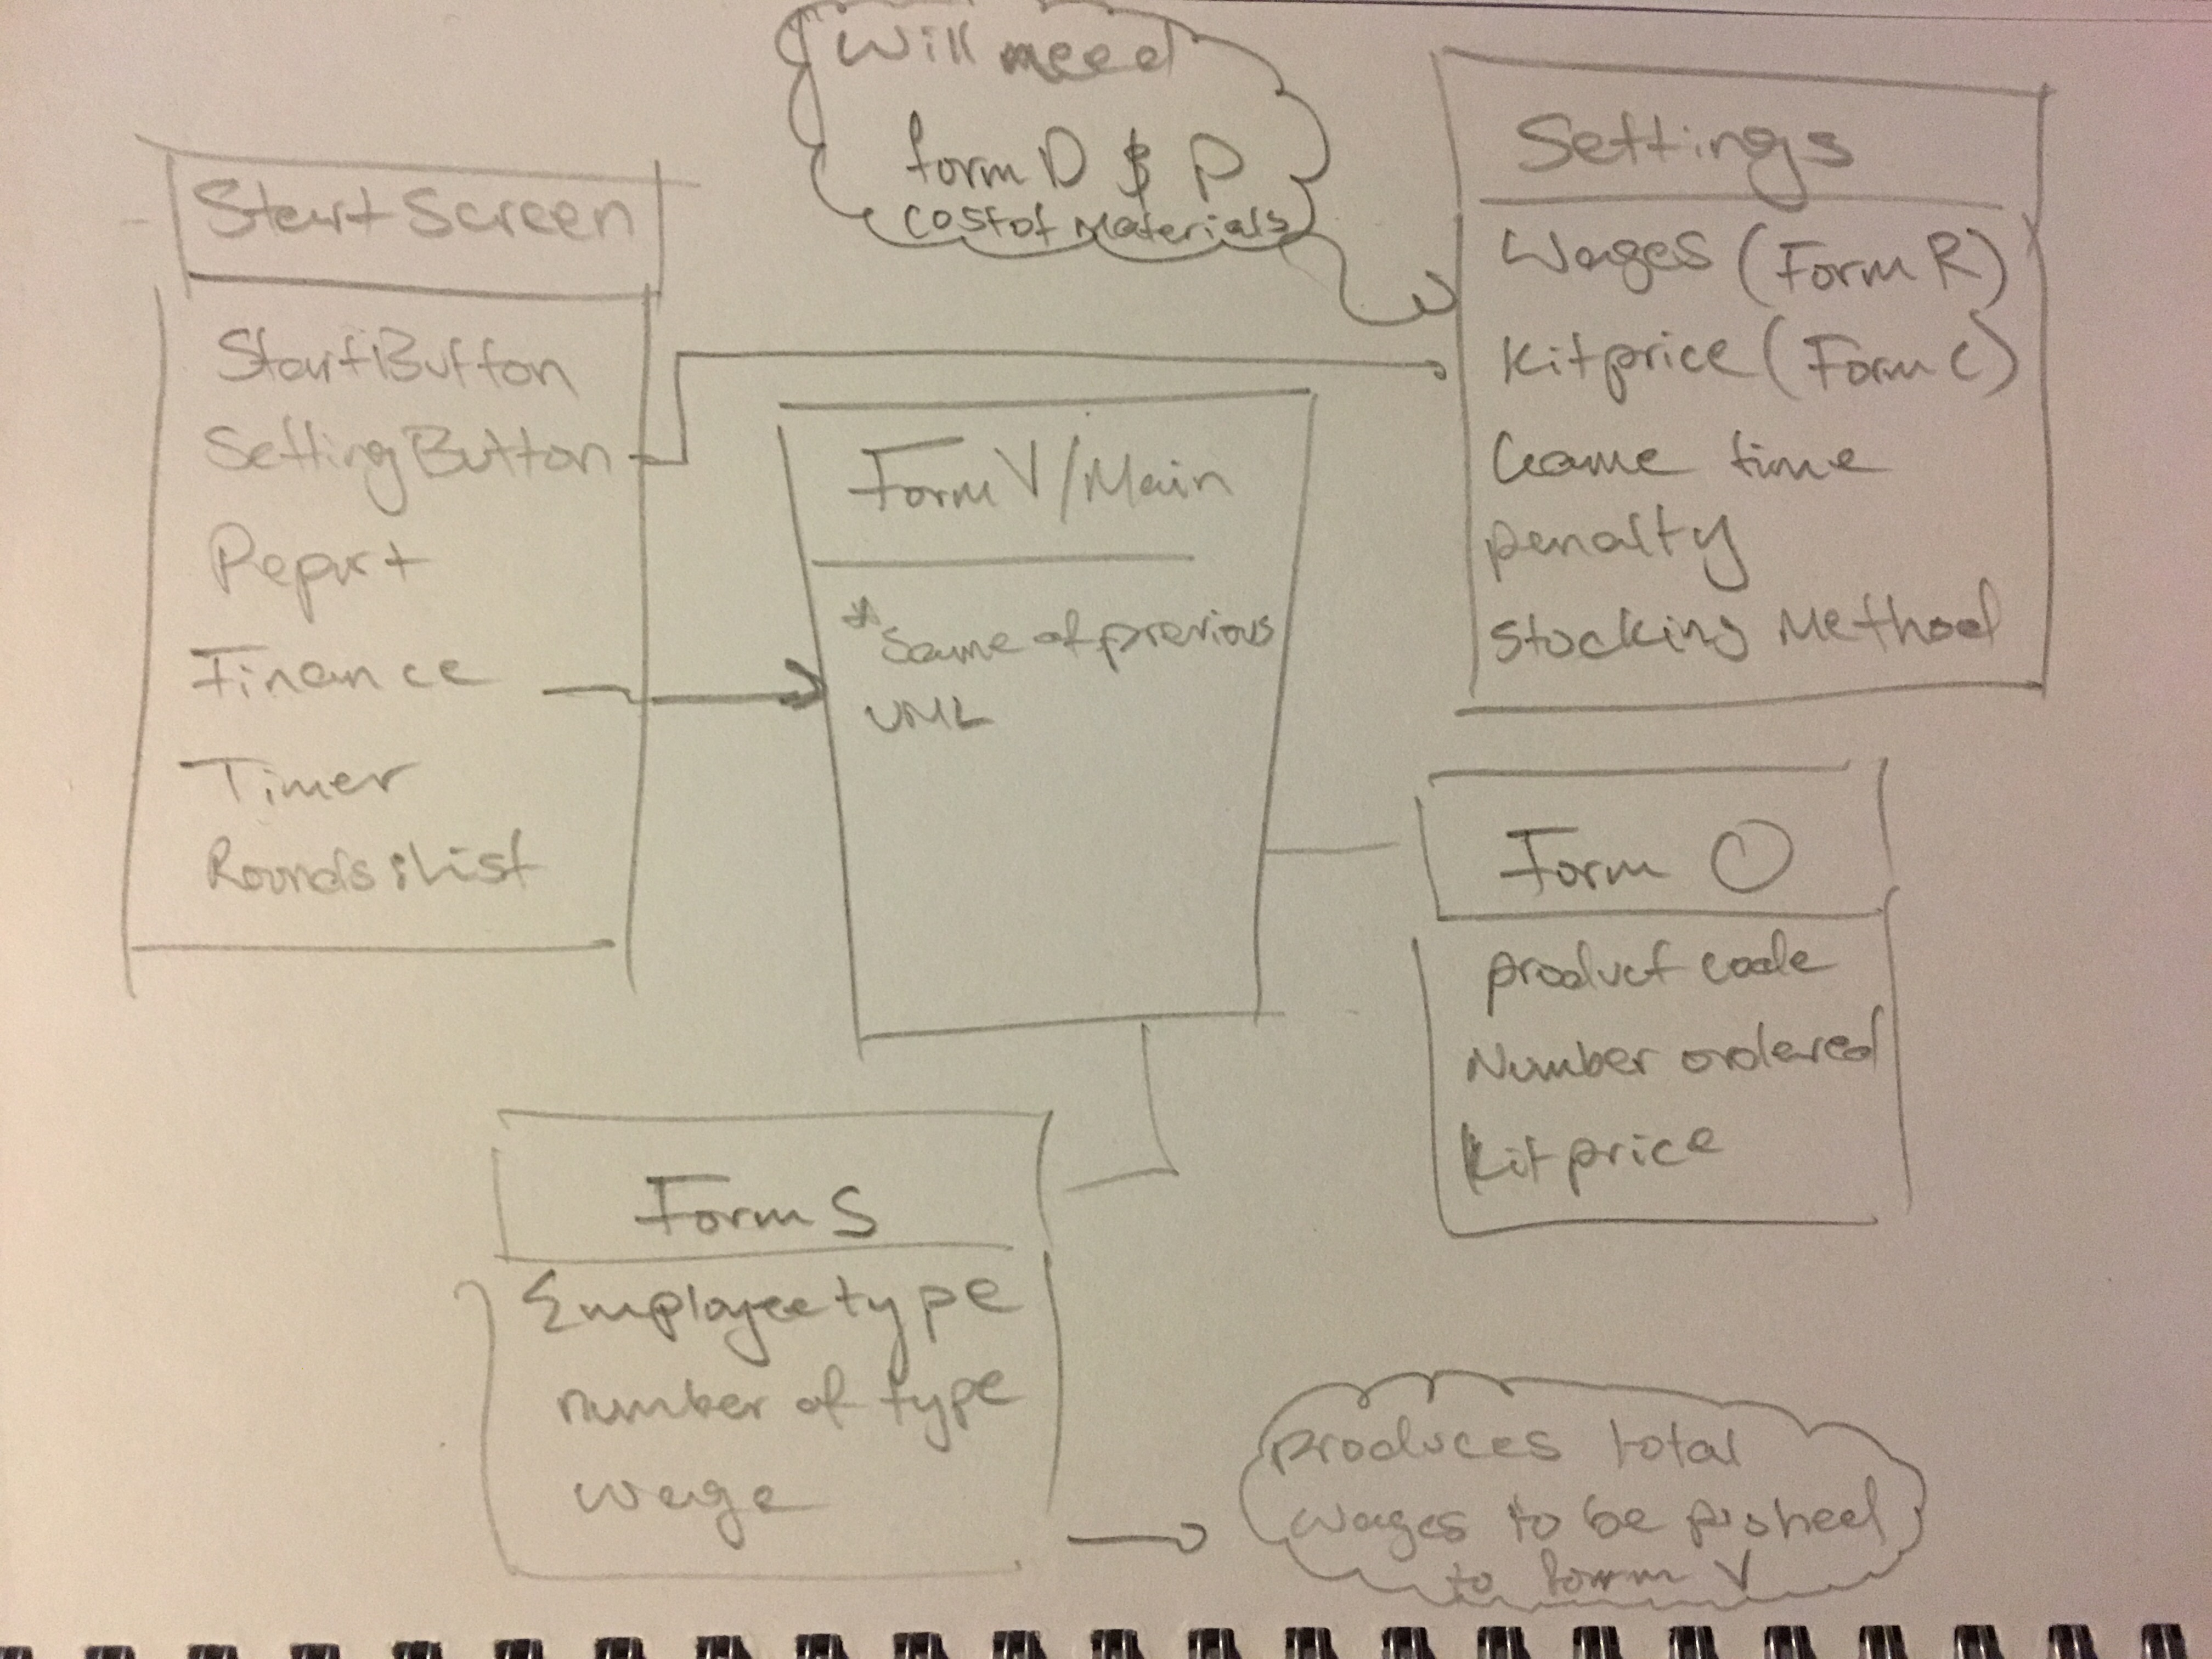
\includegraphics[width=9cm]{figures/class}
\end{center}
\caption{An early class diagram}
\label{fig:agilemethod}
\end{figure}


Shown in \hyperref[fig:class]{Figure 1} is one of the rough class diagrams the team drew up in the early stages of development. This diagram and others liked it enabled the team to effectively plan the design of the application.

\subsection{Wireframes}
After the second meeting with the client, the team chose to create some simple low-fidelity wireframes (shown below) so that we could demonstrate to the customer our idea of what the application would look like and get their feedback on the design. This technique enabled each team member to showcase their ideas and allowed us to take the best ideas from each design and merge them for the wireframe shown to the customer. It was then agreed in a meeting with the customer that a medium to high fidelity wireframe should be drawn up so that both the customer and the team could get a better idea for the desired look and feel of the application. See \hyperref[fig:wireframes]{Figure 2} for wireframes.

\begin{figure}[!h]
\centering
\subfloat[]{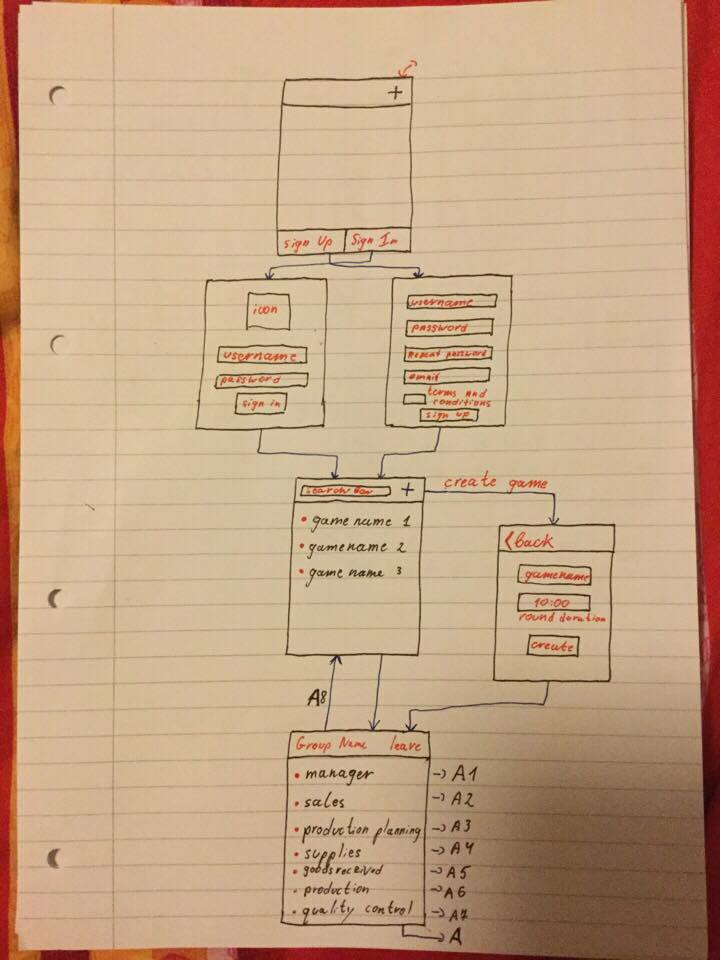
\includegraphics[width=6cm, height=7cm]{figures/wiref1}} 
\subfloat[]{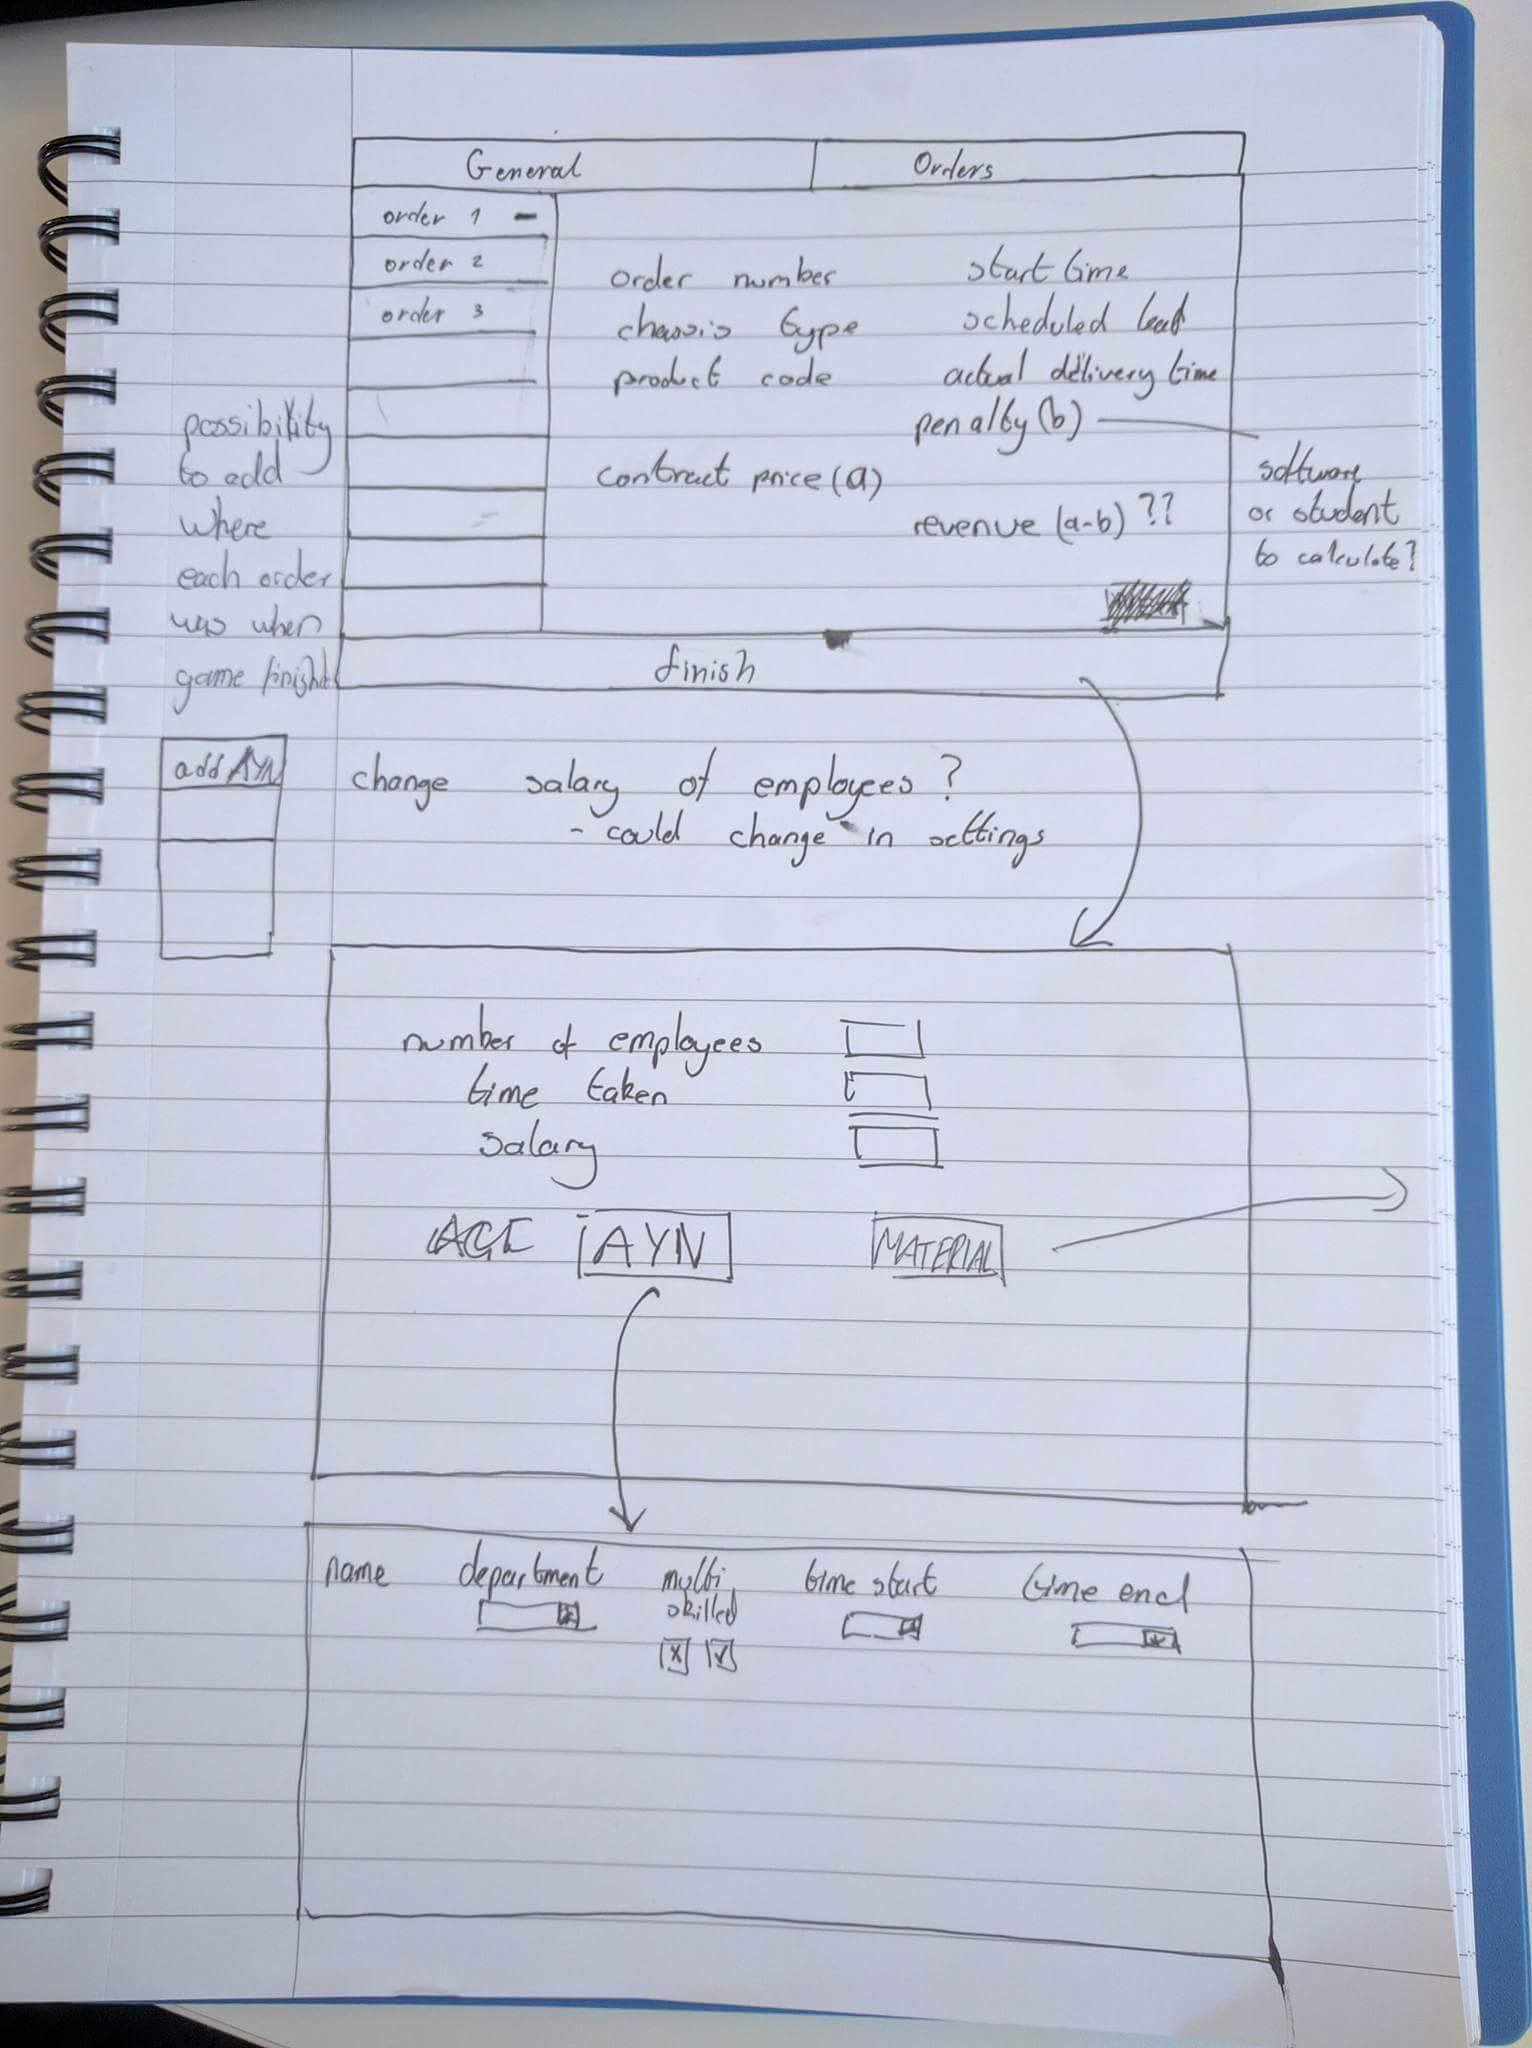
\includegraphics[width=6cm, height=7cm]{figures/wiref2}}
\caption{Two of the team's early low fidelity wireframes} 
\label{fig:wireframes} 
\end{figure} 



\subsection{Development Estimation}
Estimating the time taken to complete different stages of the development was one of the major challenges the team faced. Quite early on in the project, the team decided to use sprints as a development aid. (See \hyperref[fig:estimation]{Figure 3a} for an outline of the team's sprint.) The initial sprints, however, never met all of their objectives. This was mainly due to a lack of experience of both developing this kind of application and of small team development resulting in the team overestimating what could be achieved in a week. At the end of each sprint, the team reviewed the sprint and it soon became apparent that the developers needed to better assign tasks. As a result, in later stages of development, the team often met most if not all of the objectives set out at the start of each sprint. The use of sprints significantly benefited the project's productivity, it allowed the team to break down the large task of developing an application from scratch into small and manageable tasks, enabling steady incremental progress.

The team also used retrospectives to evaluate the status of the progress. (See \hyperref[fig:estimation]{Figure 3b} for one of the team's retrospectives.) The retrospectives allowed the team to identify both effective strategies and the areas of improvement. Furthermore, retrospectives allowed the members to express their needs, likes, and dislikes of anything ranging from meeting times to coding to the management of the team.

\begin{figure}[!h]
\centering
\subfloat[]{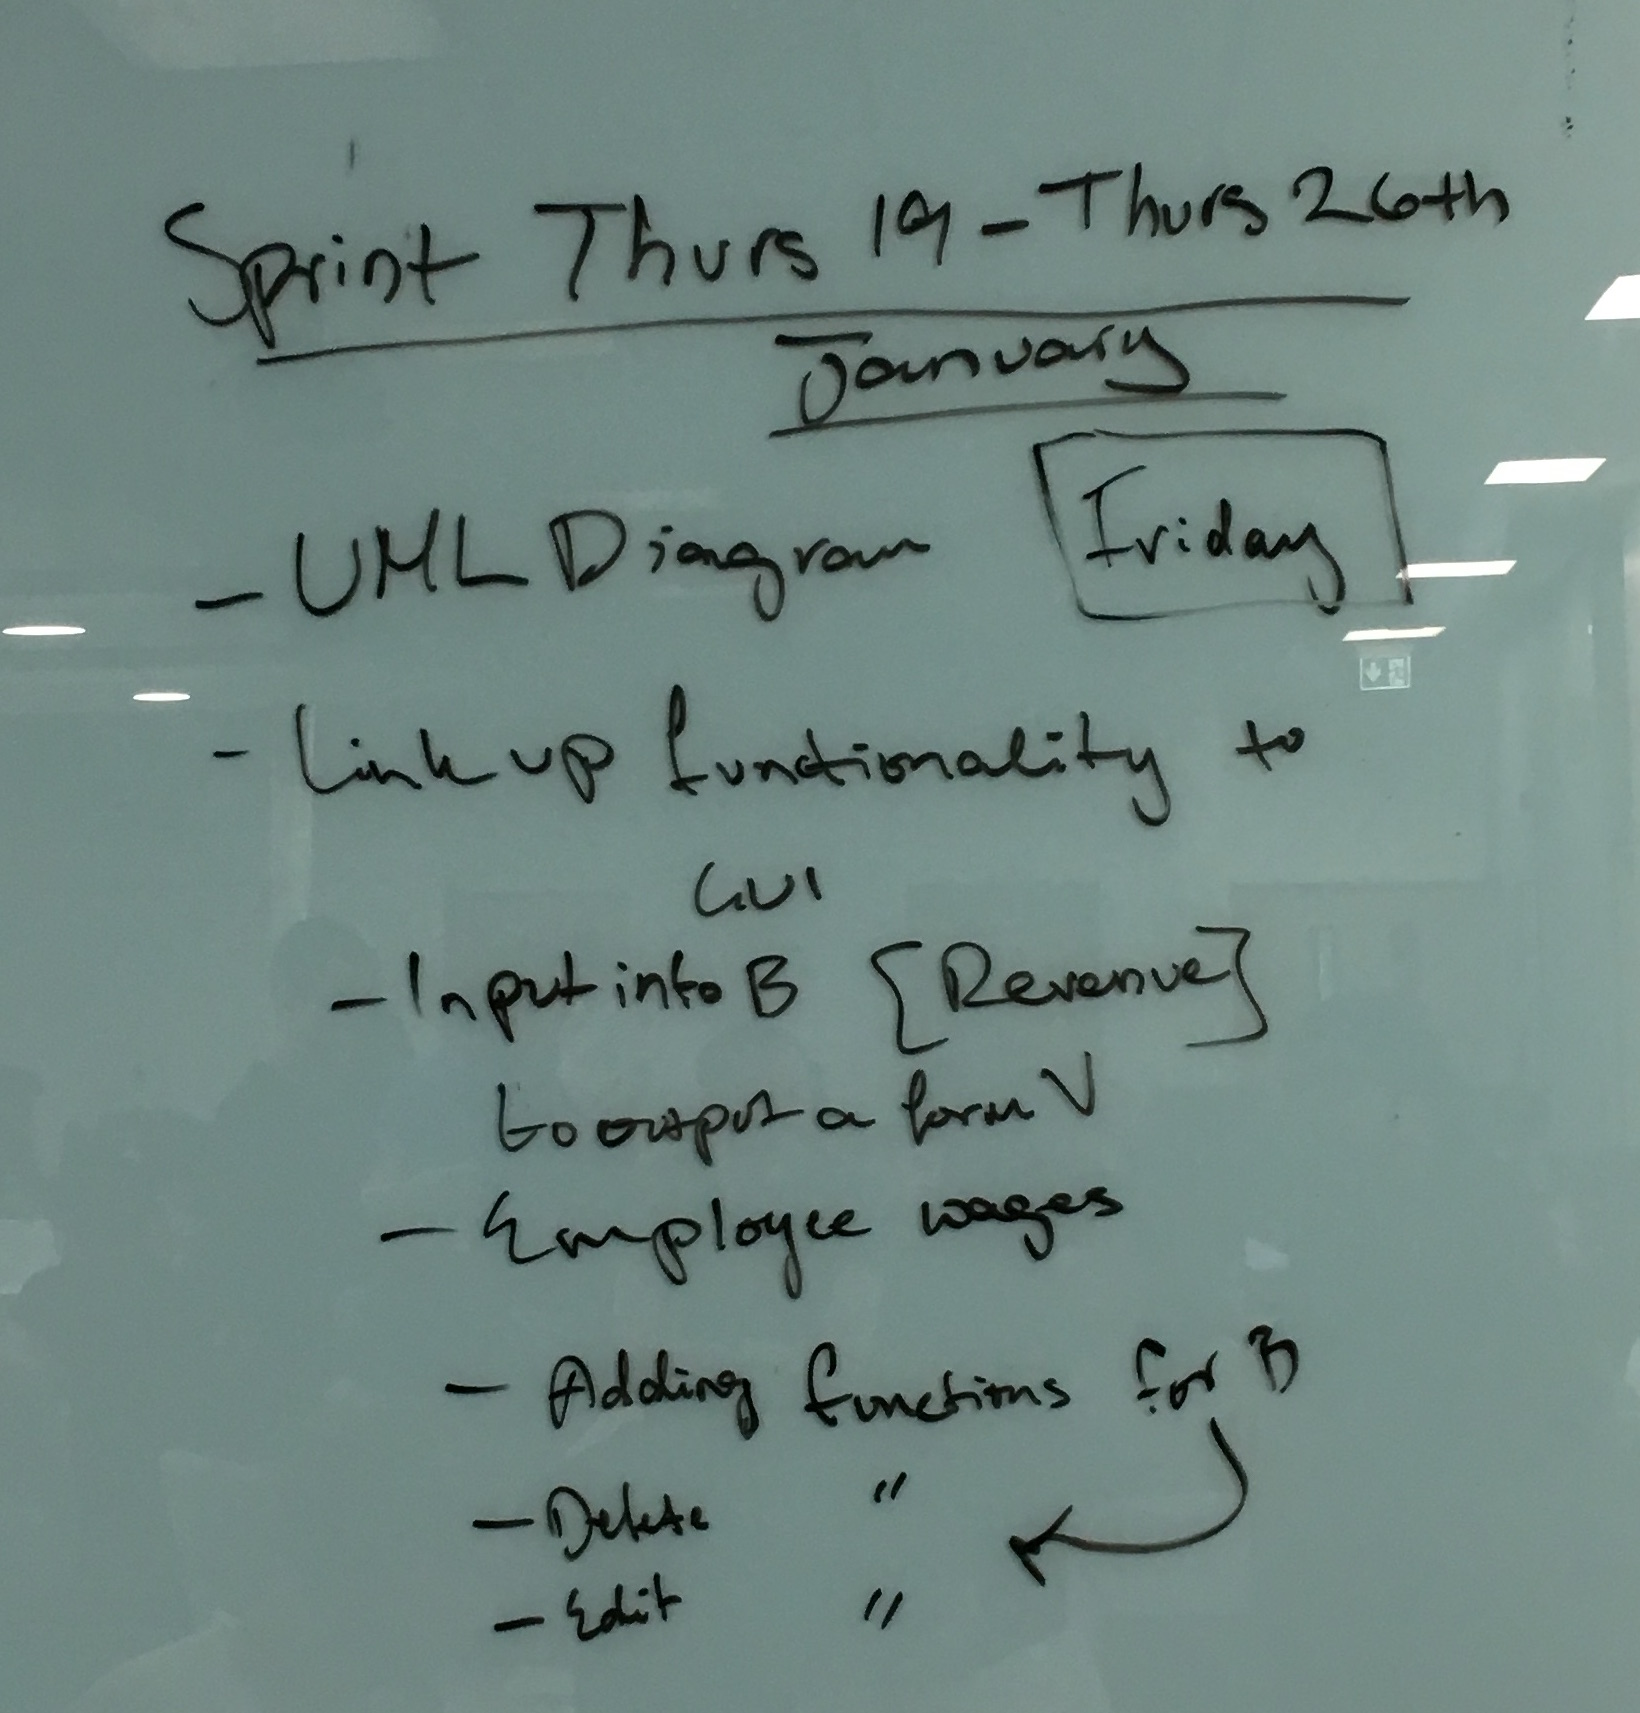
\includegraphics[width=6cm, height=6.5cm]{figures/sprint}} 
\subfloat[]{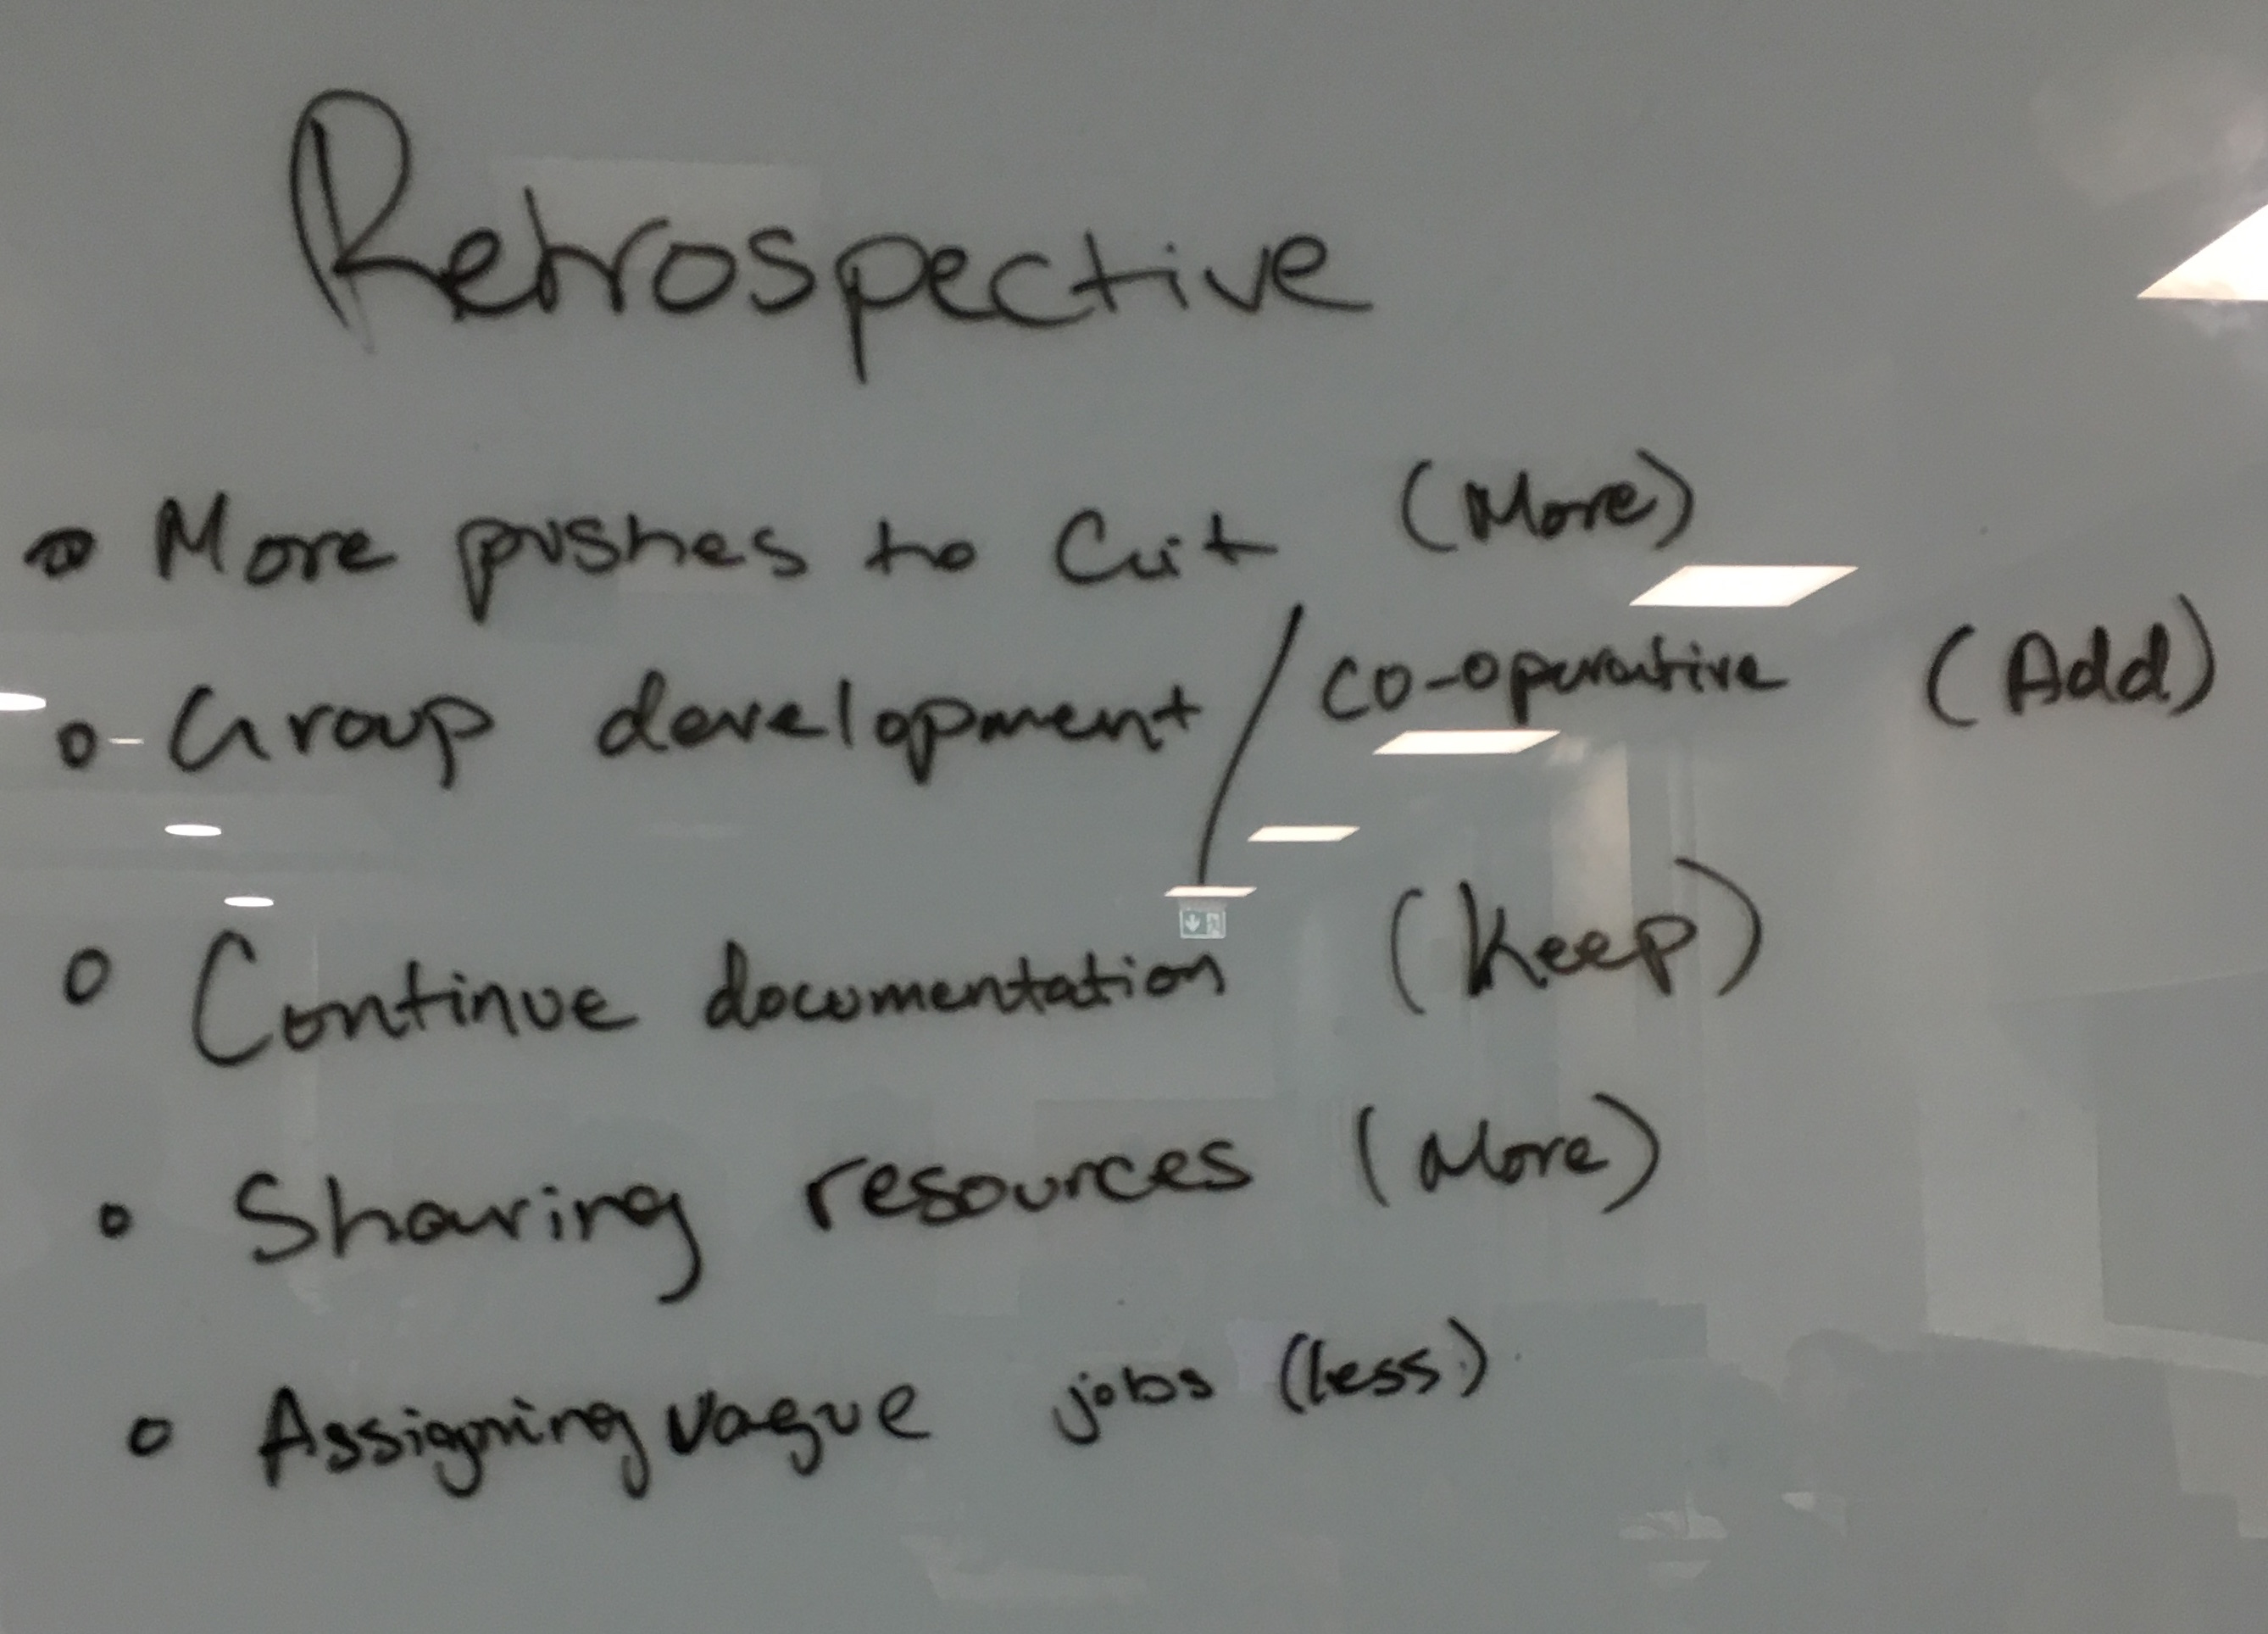
\includegraphics[width=6cm, height=6.5cm]{figures/retro}}
\caption{An example of one of the team's sprints (a), A retrospective on preceding sprint(b)} 
\label{fig:estimation} 
\end{figure} 


To help with planning a development timeline for the overall project, the team drew up a \hyperref[fig:gantt]{Gantt chart} shown below. The chart allowed us to clearly define the milestones that we wanted to achieve at different points in time. This level of planning was necessary to ensure that the project deliverables were ready on time.

\begin{figure}[!h]
\begin{center}
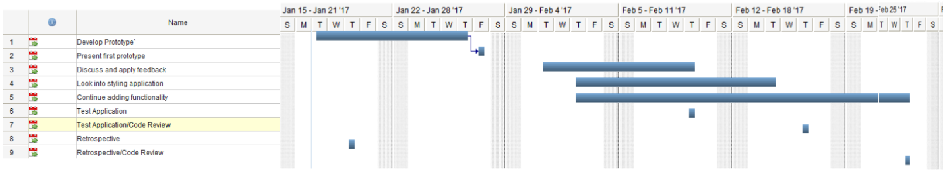
\includegraphics[width=9cm]{figures/gantt}
\end{center}
\caption{Gantt chart for overall development timeline}
\label{fig:agilemethod}
\end{figure}


\subsection{Peer Programming}
One practice which all team members engaged with was peer programming. Peer programming involved usually two team members working together on one particular problem, one coding, and the other watching and suggesting improvements. This was normally done during team programming sessions, in particular, during sprints to help tackle difficult tasks, catch typing errors and suggesting debugging choices. During these sessions, the team was able to solve problems much quicker and make substantial progress adding additional features nearer the end of development. Furthermore, peer programming helped the understanding and development of another team member's code. With different coding styles within the team, peer programming helped by having another opinion on the code that had been written and the code that was being written together. 

The team did not start peer programming until the first sprint as coding was mainly done individually. Once the team realised the benefit of coding together, peer programming became a regular occurrence during sprints and often outside team meetings when members would meet to tackle their individual tasks together.

\subsection{Continuous Integration}
The team used built in Gitlab integration tools. Since the members of the team were inexperienced with continuous integration tools prior to this project, it required some learning before the tools could be fully exploited. Inexperience and unfamiliarity were the sources of reluctance to continuously push the code to Gitlab. What is more, initially, the members preferred to use a messaging application to send their code directly to each other. However, it did not take long for the team to realise that professional software development required a more sophisticated method of code sharing.

Once the members familiarized themselves with basic git commands, they utilized branches. The code development was distributed to a small number of branches which were then merged to the master branch, once individual development stages were completed. The master branch served as a backup in this project whereas most of the development happened in a ‘development' branch. Others were used to experiment with additional, low priority functionality.

In order to make sure that unintentional bugs would not be pushed to a branch the team utilised automatic build testing, i.e. upon pushing, the code was checked to see whether it compiles and only accepted if it did. The team did not use a more elaborate automated testing because as discussed in the Testing section, the nature of the project required different testing methods.

\subsection{Tracking}
Gitlab built in tools were used to track team progress and plan future tasks. Gitlab's capability of opening issues allowed the team to create a record of the tasks for the project. Each issue could have custom labels attached to indicate a theme and priority. In addition, the tasks could have weights assigned to indicate corresponding estimated time to complete the task. Once the task was completed, the team was able to look back, evaluate the work done, and close the issue.

Tracking proved not to be a difficulty in the project. The team had a dedicated member to make sure that the issues were opened and maintained as required. However, it did take time to get accustomed to using the full range of the issue attributes (e.g. labeling). At first, the team incorrectly used weights to indicate how important each issue was and had no labels on each issue. This was due to the lack of experience within the team using Gitlab and issue tracking. Issues team members opened were vague and had little detail in the comments which in some cases caused delays as the assignees might not be fully informed of the scope of the task.
 
Supervisor feedback prompted the team to make changes to how tracking was used and set a standard within the team of how each issue must be opened and laid out. Development quickly picked up after these changes as team members were able to close issues in their own time without waiting to discuss any further details. Labels were set up to indicate the priority and subsection of each issue. For example, ‘high priority' and ‘code development'. The team then used weights correctly to indicate how long each issue expected to take. This resulted in team members being allocated equivalent workload. Another change the team made to issue tracking was referencing the commit to their respective issues.

%==============================================================================
\section{Meetings}
\label{sec:meetings}

\subsection{Group Meetings}
\subsubsection{Requirements Discussion and Delegation}
Group meetings were a key element in the success of the project. The primary role of these meetings was discussions of the requirements of the project and to delegate tasks to each team member. This aspect of the development process took up an extensive amount of the time. Initially, the meetings lacked structure and this lead to the discussions occasionally focussing on low priority problems or going off topic. However, the team quickly identified this issue through a systematic retrospective. To tackle this problem the members started to identify key talking points for the meeting at the start of each meeting, allowing the team to effectively focus the attention on what was believed to be the priorities of the project. As a result, the meetings became more productive and the developers were able to focus more time on actual development of the application. This method of keeping team meetings focussed on the important issues was effective, however in retrospect making a formal agenda prior to each meeting would have been the best solution for keeping meetings structured.

\subsubsection{Progress Discussion}
The meetings were also used to track the progress of the project and to plan the next sprint. As each team member was developing different parts of the application separately, reporting the progress of each member was important for keeping the project on track and effectively planning what had to be done. Making the decisions about task delegation as a group allowed the team to effectively take advantage of each member's strengths and ensure everyone was comfortable with their workload. In the early stages of the project, the tasks set out for each sprint were fairly large and vague. As a result, few of the objectives for the early sprints were ever met. The team identified this issue early on and quickly started making sprints made up of many small and specific tasks. This way each member could be allocated several small tasks in each stage, making it easier for the team to prioritise important tasks and ensure they were completed by the set deadline. This change demonstrated that sprints made up of small, easily achievable tasks are more effective for making good progress than sprints with fewer, larger tasks.

\subsection{Client Meetings}

\subsubsection{Requirements Elicitation}
The team met with the clients on various occasions. The main focus of the meetings, especially in the early stages of development but continuing throughout, was requirements elicitation. As mentioned previously the team took part in a live demonstration of the game to gain a better understanding of the requirements. Every later meeting was partly dedicated to gathering new development requirements of the application. This ongoing requirements gathering continued up until the final iteration of the project. An issue the team faced was clarifying requirements with the customer as the client was not always decisive about the features to be implemented in the application. This made the continual requirements gathering essential as the customer's view of what the application evolved throughout the course of development.

\subsubsection{Progress Reporting}
Reporting the progress to the customer was primarily done through face to face meetings. As previously mentioned the team faced difficulties in ensuring the time spent meeting the customer was used effectively. In part, the lack of efficiency was due to the fact that in the early stages of the project, planning took most of the time as opposed to demonstrable application development. Furthermore, a large amount of effort was required to understand the game itself and what was exactly required of the application. As discussed above the team adopted a top-down design approach to overcome this issue. This allowed the team not only to give the customer an idea of what the application would be like to use but also receive feedback which would keep the development focused. Thus, the importance of visual aids in the effectiveness of progress reporting when dealing with a non-programmer client was soon evident.

%==============================================================================
\section{Communication}
\label{sec:communication}

\subsection{Group Interaction}
The main means of communication were face to face meetings and social media. The team had a Facebook group which was regularly used to organise meetings and to report progress made in between meetings. However, it was the group meetings that most of the discussion and communication between team members was done. It was in these meetings that the team made the most progress on development of the application and it was identified in a retrospective the team carried out that having more group meetings would significantly benefit the development effort. This allowed developers working on different elements of the application to more closely coordinate their work making the integration of different parts of the product much easier. These group coding meetings were highly productive and in hindsight, the team should have exploited this development technique much sooner in the development process.

\subsection{Client Communication}
All communication with the client outside of meetings was done through email. The team set up a joint email account which was used to contact the customer between meetings. However one of the main issues the team faced was the promptness of the client's reply. The customer was always very busy and as a result getting in contact with him proved difficult. To mitigate this problem the team learned to email as far in advance as possible so as to increase the chance of getting a timely reply. In addition, an effort was made to look ahead in the project development so that issues that may arise in future could be foreseen and discussed in earlier meetings, thus reducing the number of meetings but increasing the efficiency. This issue highlighted the importance of using face to face meetings with the customer as effectively as possible so as to reduce the need for email communication. Through a retrospective the team identified more face to face meetings with the customer was something the team should pursue and so an effort was made to accomplish this.

%==============================================================================
\section{Testing}
\label{sec:testing}
The team ensured sufficient testing by devising the following strategy. First, since code errors of GUI development were clearly visible upon running the software, the team required no specific test cases. On the other hand, each team member was required to run the program and navigate the GUI until certain that implementation was correct before pushing their code to git. Additionally, each team member was required to run the program and make sure that it ran as expected immediately after pulling the updates from git. Such strategy allowed the developers see which code is correct and which parts of GUI still required attention.

In support to GUI testing method, the team held several code review session, where team members had a chance not only to familiarize with each other's code but more importantly identify bugs and general code weaknesses. Moreover, the team was able to give suggestions for improvements. The code reviews did not prove to be very effective finding issues in the code as again, given the nature of the project, the GUI would either be working correctly or not working at all. On the other hand, code review proved to be extremely helpful assisting the members who were stuck or generally sought advice.

The second step in terms of testing was developing JUnit test cases to identify existing functionality bugs. Since the product was characterized by only basic data analysis (adding and subtracting numbers), only several JUnit test cases were created. Nevertheless, regardless of the limited amount of test cases, the test suite helped to identify and eliminate a number of calculation and data retrieval bugs. Therefore, JUnit testing proved itself to be an inseparable part of product development.

Lastly, it was negotiated with the customer to have a full run-through of the game to test the completed product in action. The real-time product testing proved to be exceptionally valuable. Not only the team was able to see whether the software managed to perform in game tasks but also observe how the application coped when the game turned unexpectedly (i.e. was interrupted, reset, fast-forwarded, etc.). This simulation allowed the team to makes sure that both the program operated correctly and was flexible enough to handle unpredictable playtime issues.
%==============================================================================
\section{Code Development}
\label{sec:development}
\subsection{Front-End Development}

To facilitate the transition from paper forms to a digital application, the team decided to make the different views as similar to the already established forms as possible. This way users could learn how to use the program faster and transfer the data from the paper forms to the application easier. See \hyperref[sec:appendix]{Appendix A} for application screenshots.

\subsubsection{Settings}
After consulting with the client, the team created the settings page so that all the game data (kit prices, game rules, products, product features, product prices and etc.) could be edited. Each of the four forms (C, D, P, and R), the game takes data and the game rules form has its own page where the data can be viewed and edited. The changes are not saved until the user saves them. If the back button is pressed before the changes are saved, the user is asked in an alert view if he/she wishes to save those changes. To ensure the security of the data, a password protection for this section was created, the user has to enter the password every time they wish to enter the settings page.


\subsubsection{Game}
After starting the game, the user has the ability to go back to the main menu, save and load game data, add rounds to the current game, generate a report for the students, and open a particular round. When the game first begins there is only one round added. The user has the ability to add more (the maximum number of rounds for all games is set in the settings page). This design choice was dictated by the customer concerns of not having enough time to play the full game in certain cases. Therefore, instead of having a set amount of rounds, each one is constructed after selecting "Add round".

As mentioned above each game has the possibility of being saved and then loaded at a different point in time. This allows the customer to stop playing a game, and if they wish to continue playing it later. Moreover, the application allows generating a report -- the features the customer desired the most. The report facilitates the students making conclusions, as each of player can easily be handed a copy of game data. Each report is generated with the data from the different rounds in the current game. It is split into sections, each corresponding to a different form in all of the rounds.


\subsubsection{Rounds}
Each round resembles \hyperref[fig:FormV]{form V} provided by the customer. No data can be edited here, as this page functions as navigation to the main sub-forms filled by the user and as a representation of all the data inputted so far. This was done, to reduce the amount of data entered by the user and to automate the calculations from the different sub-forms. Time efficiency while inputting data was was no the key customer requirements.

\subsubsection{Forms}
As mentioned before, the forms try to resemble their paper counterparts as much as possible to reduce the time a user needs to get accustomed to them. As form B requires the most input from the user, the team decided to make the process as fast as possible. This was achieved by adding auto-complete to some of the fields which required input data not from the currently played game, but from the system itself.

For \hyperref[fig:FormO]{form O}  all the data is generated by the system and the user does not need to input any data. This was done because all the data required for it is already set up in form B. Thus, even though the players are required to fill form O separately on the paper forms the team allowed the data to be transferred automatically and save users' time.

\hyperref[fig:FormS]{Form S}  deals with the permanently employed employees. The user can add new ones or delete old ones at will. Each employee requires a position and a name. This is needed to make the calculations for how much money they are paid in form V. Employee rows, whose data is left blank on return to the previous form, are not saved in the records.

\hyperref[fig:FormT]{Form T} deals with the AYN employees who are not part of the company and come to help out when there is a need for extra hands. Since they may not play the entire round, the user has to select for which how long the employee had worked, what positions he/she was hired for, and whether the employee was trained to work in multiple departments.

\subsection{Back-End Development}
\subsubsection{Java}
When the team first started the project, the decision was to choose an appropriate development language. After some consideration, it was decided that the team would use Java due to its cross-platform compatibility. This was required since the customer wanted to be able to play the game on both Macs and PCs. Additionally, since all of the team had previous experience with the language it an easy decision to make.


\subsubsection{JavaFX, CSS, FXML}
The graphical interface of the project was created with JavaFX. The team chose JavaFX because it introduced several improvements over Swing (such as the possibility to markup UIs with FXML and to theme them with CSS). Additionally, JavaFX has a cleaner and more consistent API across components, and while Swing is a fully featured and supported library at the moment, it may not be the case in the future (JavaFX is replacing Swing as Oracle's UI library for Java), which would have limited the project if additional features were required in the future.

The team decided to use FXML for the project, mostly because it required little work to implement complex views with multiple data entry points. An additional advantage of this language was that since FXML is not a compiled language, the team did not need to reload the project every time a change to the FXML was made. This allowed for faster work process and fewer distractions. Since the basic objects created with FXML do not have an elaborate styling, the team added a custom style to the project. Therefore, CSS was used to create custom styles for the different pages.

\subsubsection{Singleton, Data Structures, and System Data}
Most views in the application are created and destroyed when the user opens and closes them. Because the developers needed to keep the data throughout the entire time the game was played, it was decided to use a singleton. This allowed the team to store all the data from the many different views, and the system data in one place. It kept the data storage class concise and allowed for quick implementation changes. Additionally, because the singleton had only one instance, the team could transfer data from the different pages, without having to implement multiple functions between the different views.
 
The system data is separated in the four forms (C, D, P, R) and game rules. Since these are needed throughout the entire game their information is stored and accessed from the singleton. The first time a user requests data from one of these forms, the system checks if that data has already been loaded. If it has not then the application opens the corresponding file in the database and loads its information into memory, then it returns the required information to the user. This was done to avoid having to open and close the database documents multiple times.

The game rules data is also mapped into a hash table, since the user may only require a specific field from all the information in the table. The hashing was done through the same means as loading the data from the database files. The first time a specific field is called, the hash table is created with the name of the row as key and the value of the row as the value for the hash. After that, the specific field is returned.

All of the data from the forms is also stored in the singleton. The data from each form V is stored into an ArrayList. There are functions that allow the user to call the data, update or delete it. This allows for data to be edited even if the round is closed. With the export (save) and import (load) functionality, this even allows for game data to be edited after the program has been closed and reopened.

\subsubsection{Exportability (save) and Importability (load) of a Game}
One of the client's requirements was that a game should be able to be saved and reloaded at a later stage. To achieve this, the team used the functions for setting, getting and updating game data from the singleton to access all of the game data that was in memory at that moment, and then create four ".csv" files. The developers decided to save the data in this format as it allowed the client to have the ability to access a saved game's data, even if the user did not have the game running.

When saving the game data, it takes all the information from the singleton, changes it into a string (each ArrayList element represents a row in the ".csv" file) and then saves it to the designated file. The loading of data is the reverse process, with files being read line by line, and each line producing a different row in the ArrayList. There are four main files created after each game export (save). An additional feature, the team implemented is that the user does not have to load all four files, but as many of them as one wishes. This allows easier editing of the data (i.e. load all the forms B and V, while not getting the employee data).

\subsubsection{Controllers}
Since most of the controllers had a number of repeated functions, the team decided to create a "Base Controller", which is extensible from all of the other controllers in the application. This allowed the team to avoid code redundancy and saved time when creating many different pages. An additional advantage of this approach was that it allowed the developers to have a skeleton of each page, on which the members could quickly build the functions that were needed for the particular page.

%==============================================================================
\section{Final Product Features}
\label{sec:finalproduct}
Following the QPQ game framework a financial assistance tool was produced to tackle the client's timing problem during post round financial evaluation. The lightweight tool can perform all the computations and arithmetic required by the financial team. The application itself does not interfere with the workings of the game but only hastens the activity of the financial team.

The computational aspect is considered the main feature of the application. As mentioned, each screen mimics a form seen on the QPQ game framework. The main screen (\hyperref[fig:FormV]{Form V}) lists all the output data for the processed input data. Users are required to access each field by clicking on its respective button to access another screen (form). Within each screen there are fields for the forms required input data. Form B, where a certain order's financial details are input, such as contract price, and scheduled delivery time. This form ultimately produces total revenue seen in the round. Another screen pertains to the employee details \hyperref[fig:FormS]{Form S}). This form only requires the employee name and position, the application computes the total wage from these details. \hyperref[fig:FormO]{Form O} represents a summary of the orders input in form B and computes the total price of the materials used. \hyperref[fig:FormT]{Form T} is dedicated to holding the AYN employees details, who have their own unique wage scheme. Form V computes the profit/loss seen by that round in accordance to the above produced figures. A StartScreen has also been provided to act as a lobby between rounds. This screen consists of a start button, which generates a new round, a settings button, to access the settings page, a report generation button for export, as well as a timer button, to open a timer in a separate window, as requested by the client.

The simplicity of the tool and its close similarity to the already existing documentation, means that it requires little extra user instructions. The extent of which consists of the purpose of each form and their meaning as described by the game documentation provided by Dr. Dekkers. The application itself is small in size, portable via a physical storage unit, and has no network connectivity requirement. This means the tool is quick, simple to set-up and utilise during intensive tutorials.
%==============================================================================
\section{Conclusion}
\label{sec:conclusion}
\subsection{Conclusion}
Group software development projects tend be cumbersome and time consuming. There is a heavy emphasis on the communication of ideas to keep development intact. Agile software development processes provide useful frameworks to be able to deal with the difficulties behind group projects. The main purpose of this course was to evaluate these implemented practices while developing a functional software application to satisfy the clients' requirements.

A notable lesson to take from this study was the requirement to operate in a professional manner throughout the course. Most members, prior to the beginning, had not undertaken a professional project but rather worked individually on university assignments. The inexperience with these professional practices meant requirement elicitation, engineering, and estimation was fairly disorganised. However, after research and feedback from supervisors, it became clear to Team B how to tackle and manage development, whilst implementing agile software practices. The effects of this change were evident throughout the second half of development where clear milestones were set on a regular basis. Setting smaller detailed issues made communication more effective and development more coherent as each team member gained a better understanding of what was required of each component.

From analysing the development process as a whole, the team has learned many practices and improvements after making mistakes and learning from them. One area the members would ensure was planned and designed to stricter standards is code structure. Due to each team member having different coding styles and experience the code quickly moved away from the initial object-oriented design which was first suggested. As a team, the members did not make strict coding rules when designing the application. In hindsight, this was naive and caused some code to styled differently. A stricter design pattern, more time spent programming together, and discussion of each element would have prevented this from happening as the code would have been more organised and coherent.

Even though some sort of team difficulties occurred until the end of the project, the team agreed that communication and careful planning were integral parts of working together. And while the students had little prior experience working in a professional group software development project, a steep learning curve was felt within the team throughout the year. Furthermore, reflecting back on the process, working in a group is a skill in itself and while it took time to learn each others' strengths and weaknesses the team grew together and accomplished more as a team than they could have while working individually.
%==============================================================================
\pagebreak
\section{Appendix A}
\label{sec:appendix}

\subsection{User Documentation}
\subsubsection{Starting the game}
On entering the game, the user is given the option to go to the game lobby by clicking the "Start Game" button or the settings lobby by clicking the "Settings" button. On clicking the "Settings" button the user is prompted for a password (held by the game administrators).
\begin{figure}[!h]
\begin{center}
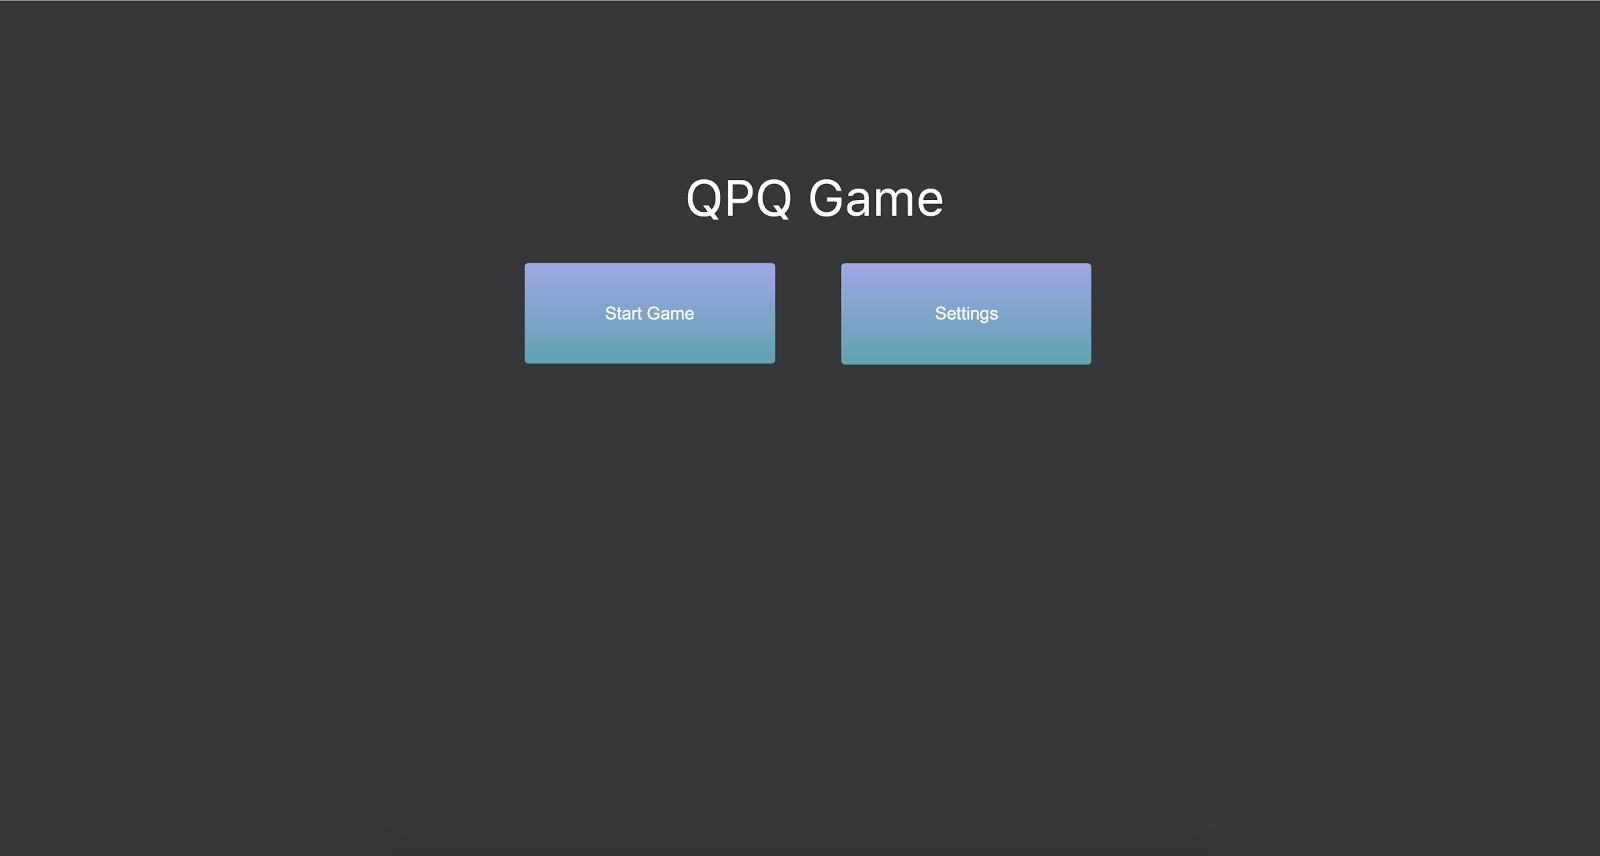
\includegraphics[width=9cm, height=5cm]{figures/startGame}
\end{center}
\caption{Start Screen}
\label{fig:startGame}
\end{figure}

\subsubsection{Settings}
\begin{figure}[!h]
\begin{center}
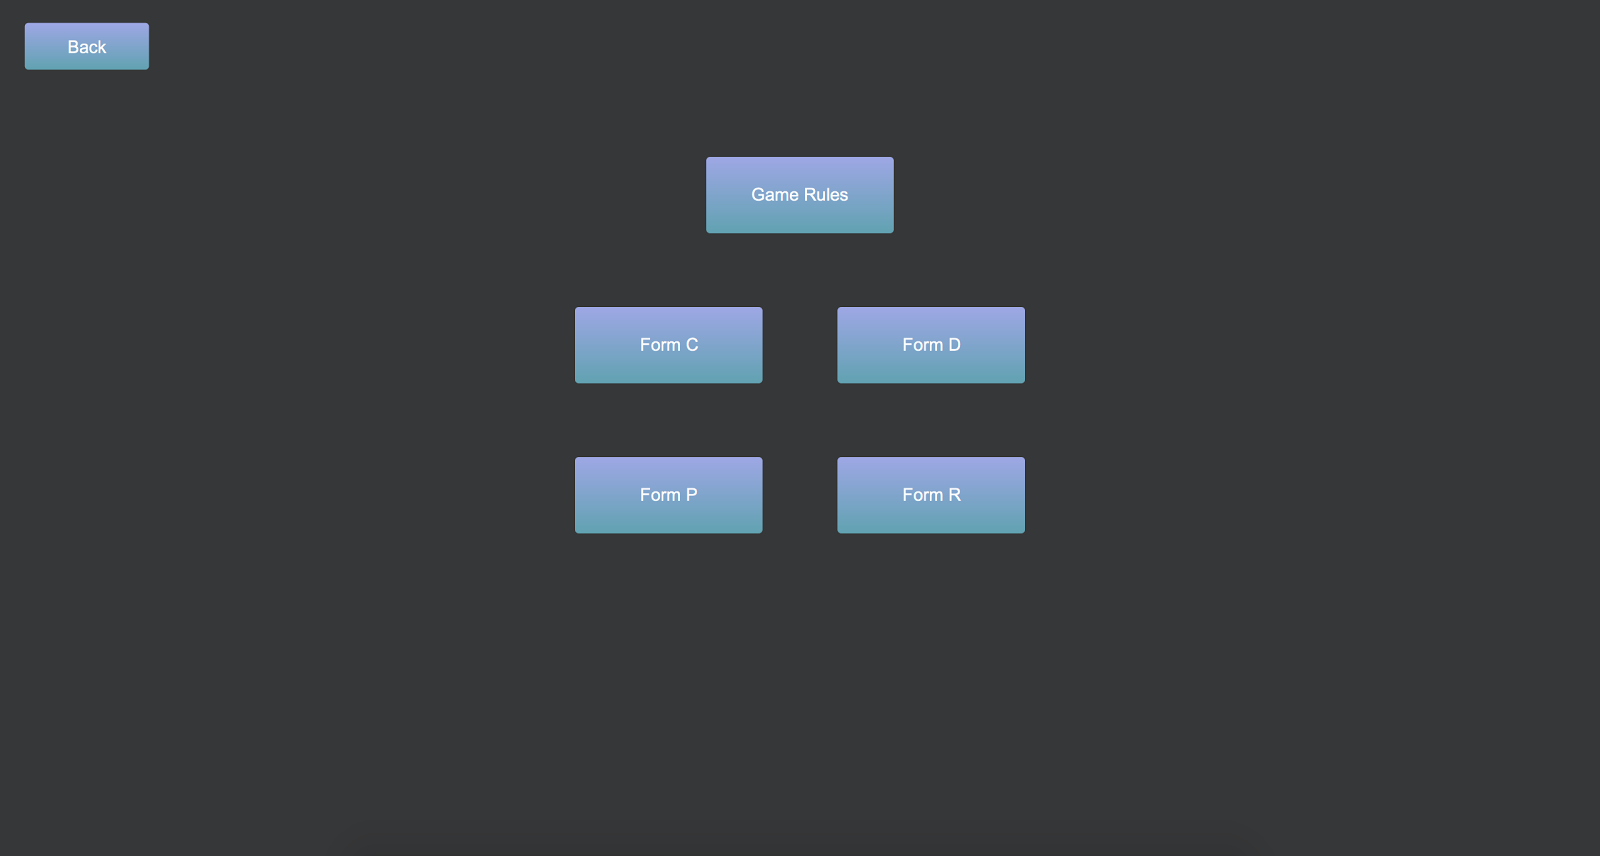
\includegraphics[width=9cm, height=5cm]{figures/settings}
\end{center}
\caption{Settings Page}
\label{fig:settings}
\end{figure}

\begin{figure}[!h]
\begin{center}
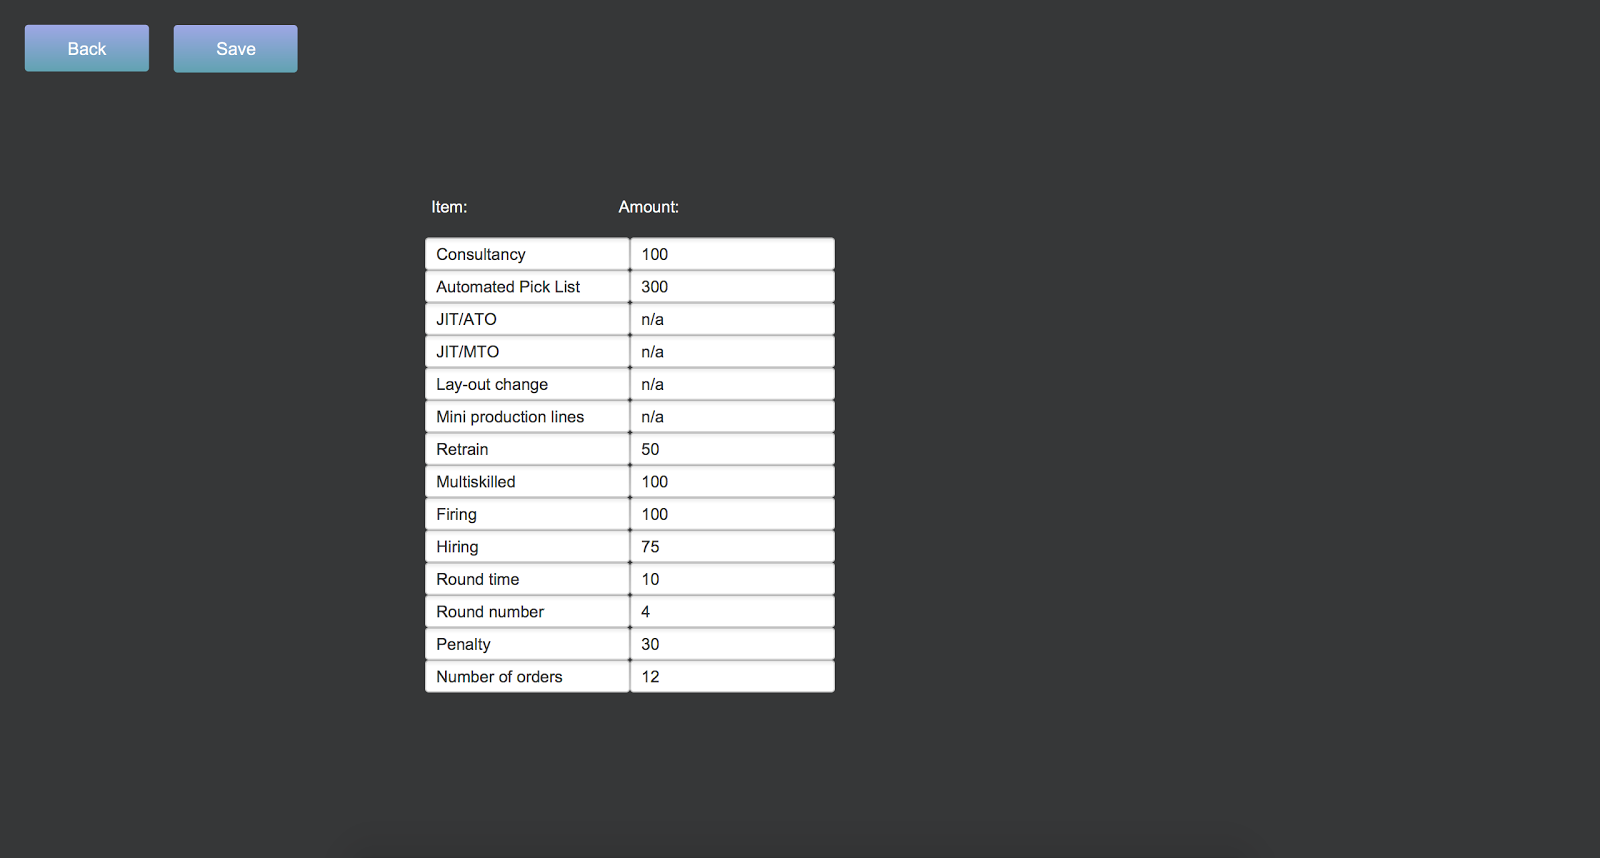
\includegraphics[width=9cm, height=5cm]{figures/settings-change}
\end{center}
\caption{Settings}
\label{fig:settings-change}
\end{figure}

The user, here, is given the option to edit game rules and in game data. 
By clicking "Game Rules" the user is redirected to its respective menu (shown below). After alterations are made the user must save the data by clicking the "Save" Button.
Form C, D, P, and R allow the user to edit data that will be used by the application to process input data against. On editing each form the user must save before exiting to confirm data is changed.

\subsubsection{Game Lobby}
In the game lobby, the user is presented with a number of option, shown below.
\begin{figure}[!h]
\begin{center}
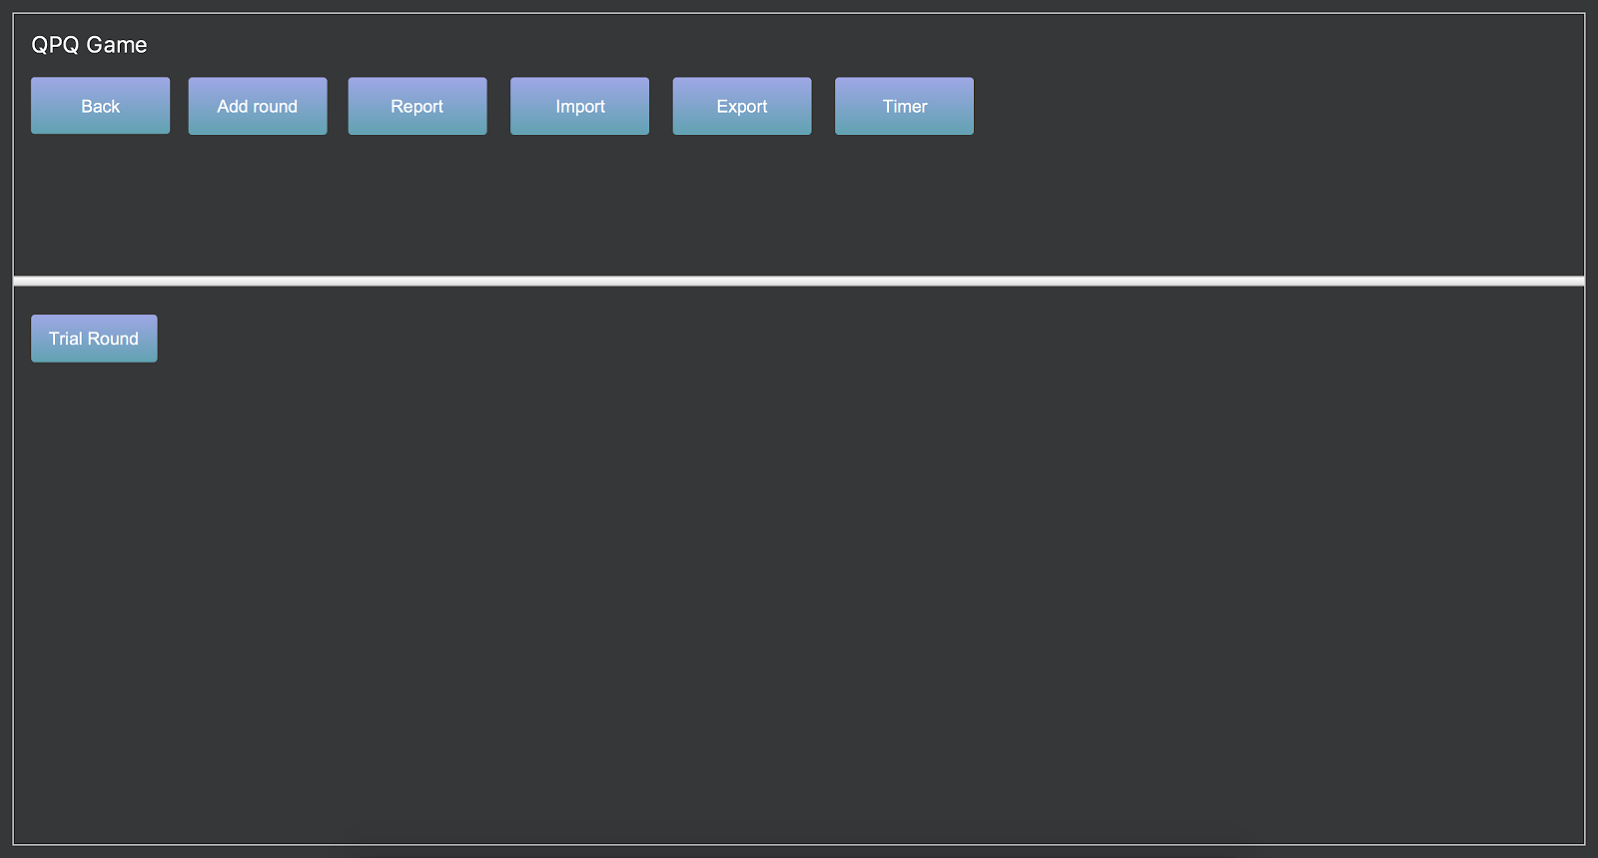
\includegraphics[width=9cm, height=5cm]{figures/gameScreen}
\end{center}
\caption{Game Screen application}
\label{fig:gameScreen}
\end{figure}

\subsubsection{Adding a round}
The user must click "Add Round" to generate a new round that will appear below the solid line as shown to the right.
\subsubsection{Saving a game}
On clicking the "Export" button 4 .csv files pertaining to data in Form B, S, T and V are generated which may later be imported through the "Import" button. No headers are present on these files.
\subsubsection{Creating a report}
The "Report" button will generate a single .csv file filled with the correct headers for all the rounds.
\subsubsection{Timer}
When the "Timer" button is clicked a new window is opened (shown below), showing a count up timer that will run for the amount of time given in game rules.
\begin{figure}[!h]
\begin{center}
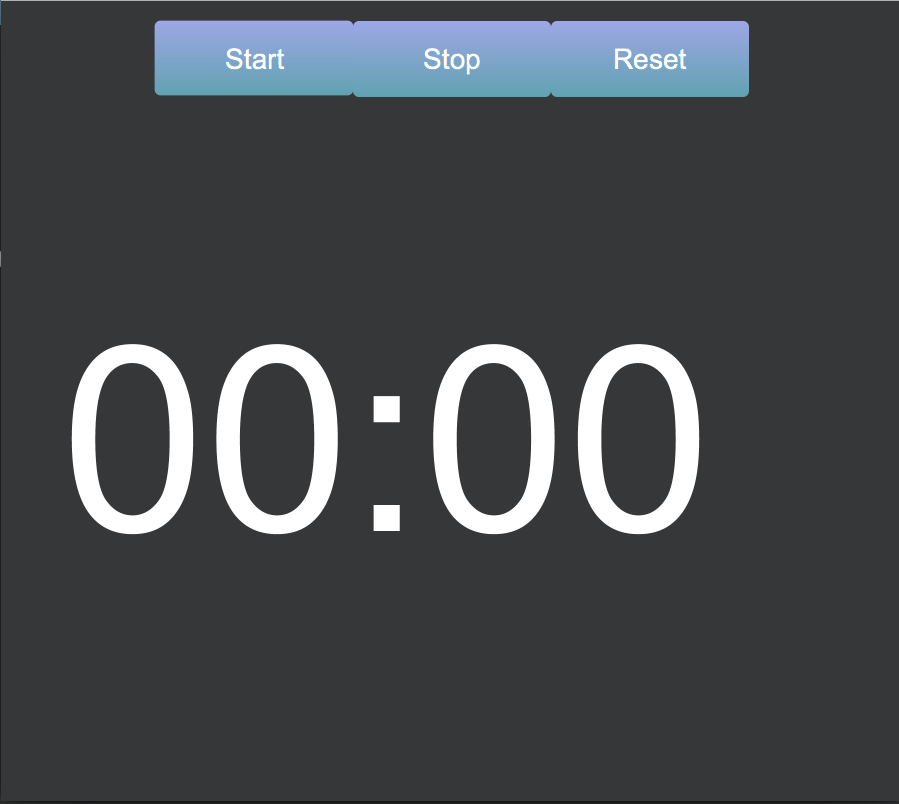
\includegraphics[width=10cm, height=7cm]{figures/timer}
\end{center}
\caption{Timer}
\label{fig:timer}
\end{figure}

\subsubsection{Adding round data}
To add round data the user must click on any of the round buttons which appear below the solid line to access the round lobby (Form V, Figure 10, shown below).
In the round lobby the user has the option to access each form, by clicking its button, and input the data related to that form. On returning to the round lobby from each form, data is auto generated and presented.
\begin{figure}[!h]
\begin{center}
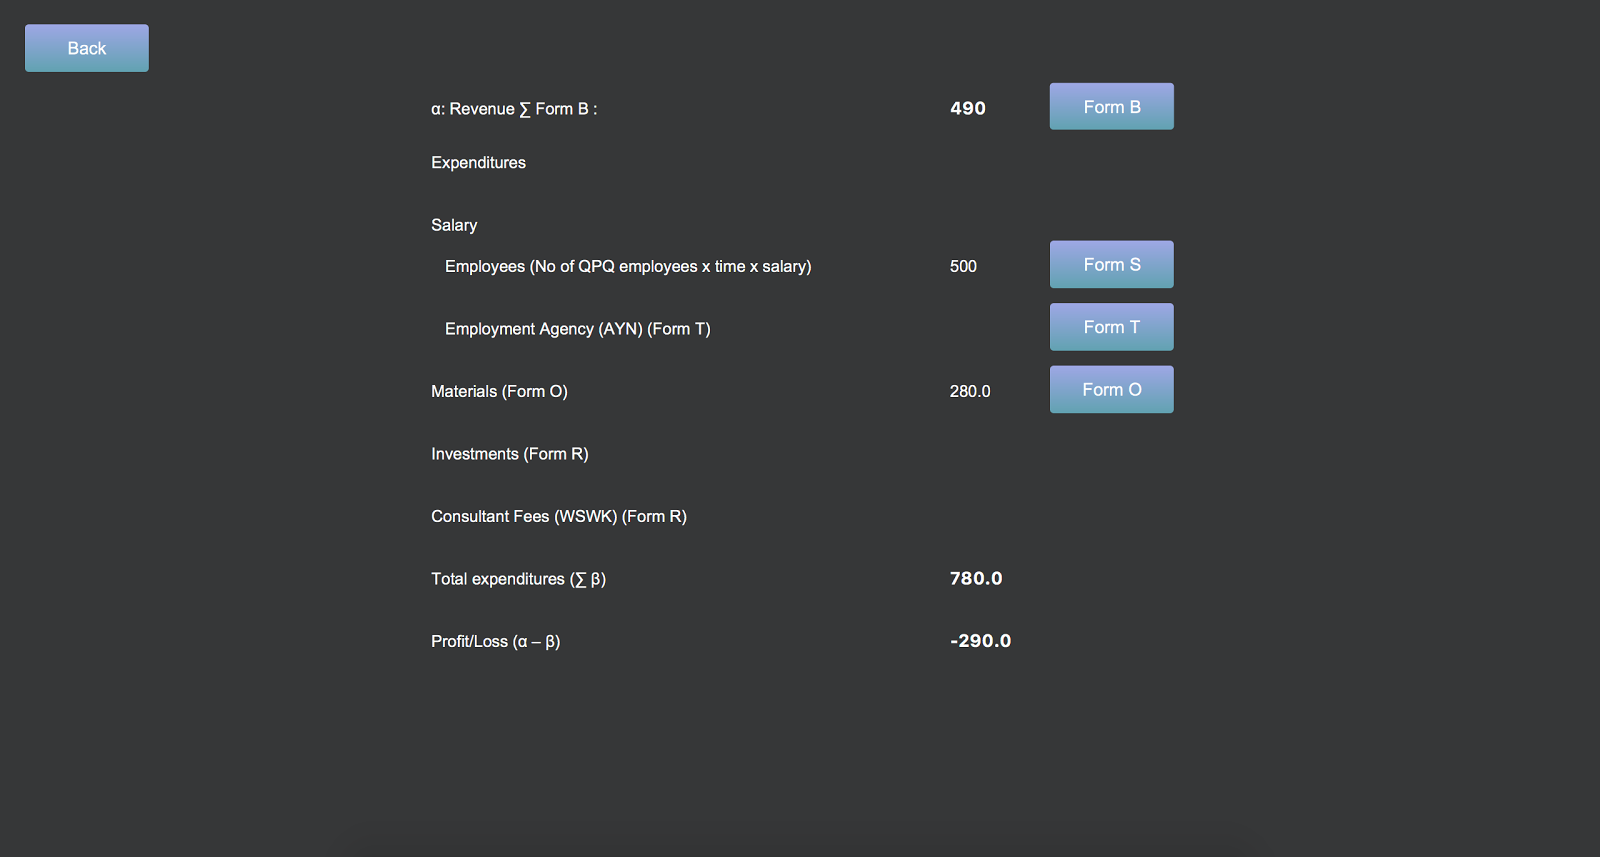
\includegraphics[width=9cm, height=5cm]{figures/FormV}
\end{center}
\caption{Form V Application}
\label{fig:FormV}
\end{figure}

\subsubsection{Form B}

Enter data correctly for each field. An example is given in Figure 11. Scheduled Delivery Time, Chassis Type, Penalty and Revenue are automatically generated. \begin{figure}[!h]
\centering
\subfloat[]{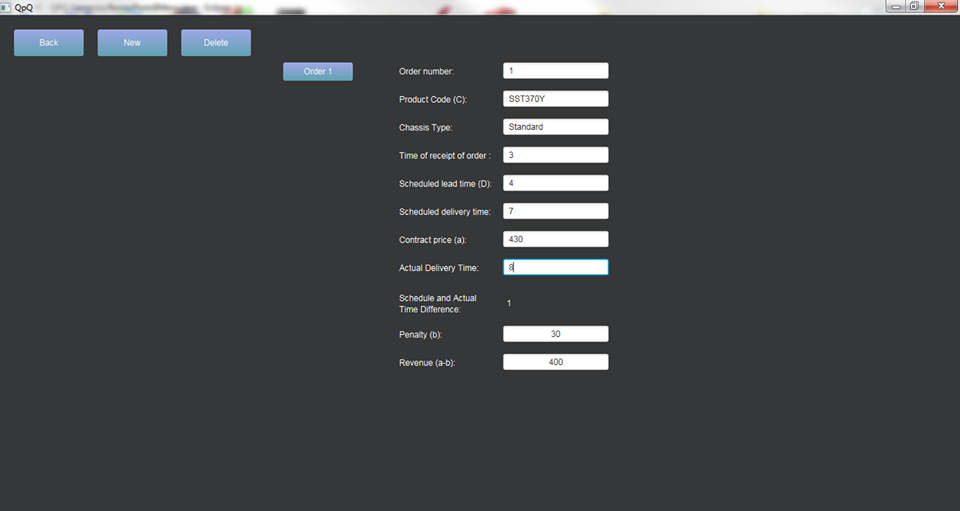
\includegraphics[width=7cm, height=4cm]{figures/FormB}} 
\subfloat[]{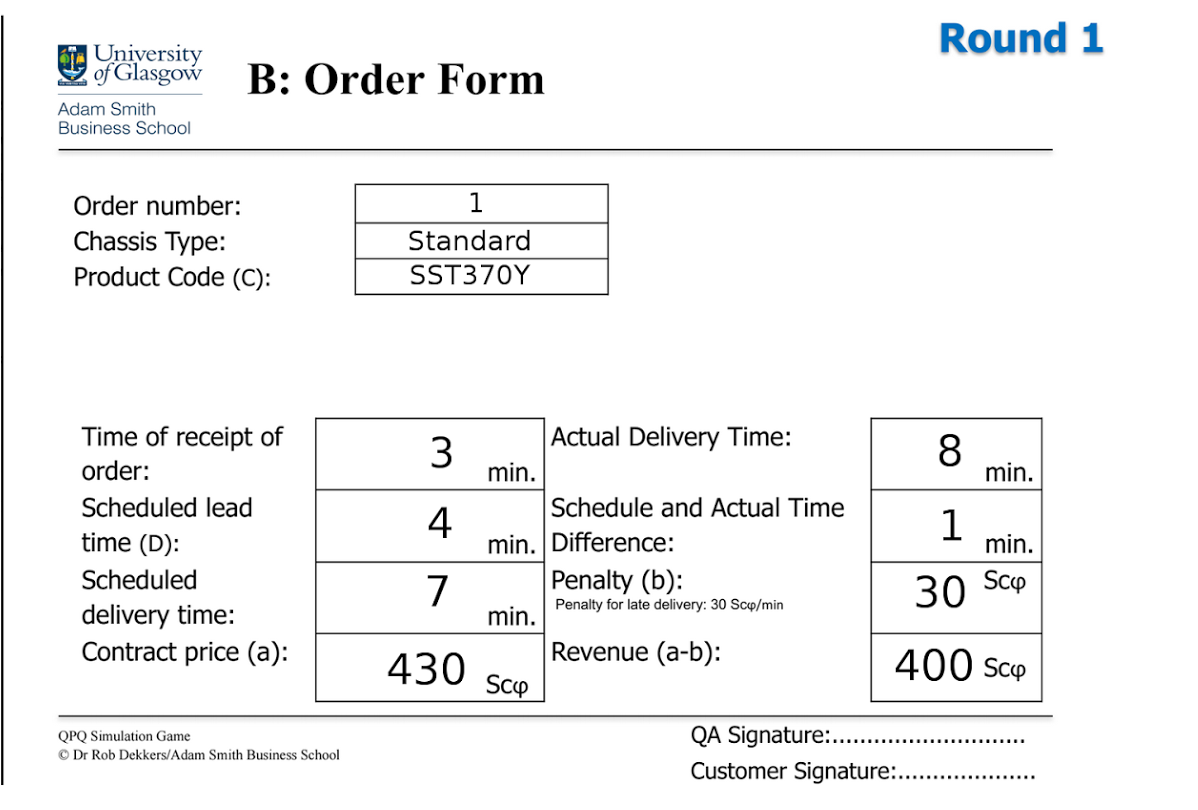
\includegraphics[width=7cm, height=4cm]{figures/FormBPaper}}
\caption{Form B}
\label{fig:FormB}
\end{figure}


\subsubsection{Form O}
The user here is presented with a summary of the orders made and list the expenditure in terms of materials. Example given below.
\begin{figure}[!h]
\centering
\subfloat[]{\includegraphics[width=7cm, height=4cm]{figures/OrderHistory}} 
\subfloat[]{\includegraphics[width=7cm, height=4cm]{figures/orderHistoryPaper}}
\caption{Form O}
\label{fig:FormO}
\end{figure}

\subsubsection{Form S}
Enter data for every employee correctly. New employees may be added by clicking "Add New" Button and existing employees may be deleted by selecting the the employee then clicking the "Delete" button. Data will save on clicking "Back". An example is given below.
\begin{figure}[!h]
\centering
\subfloat[]{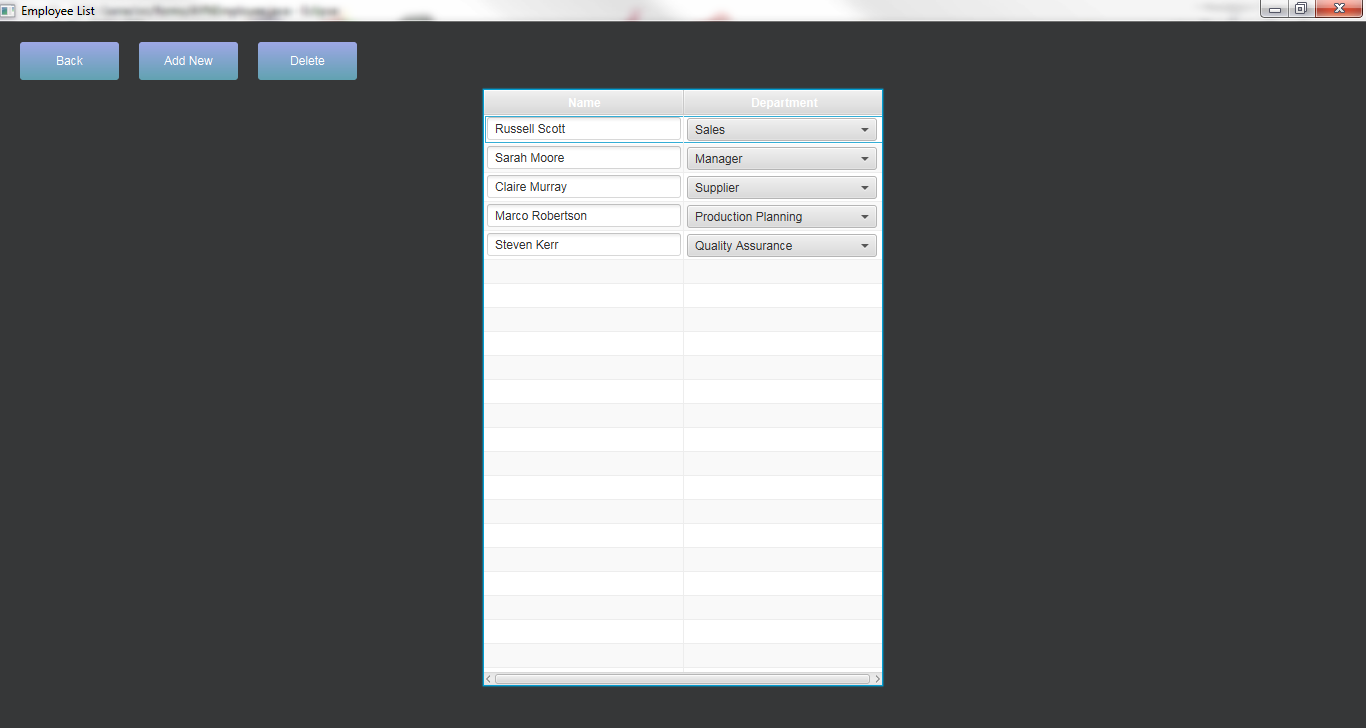
\includegraphics[width=7cm, height=4cm]{figures/EmployeeForm}}
\subfloat[]{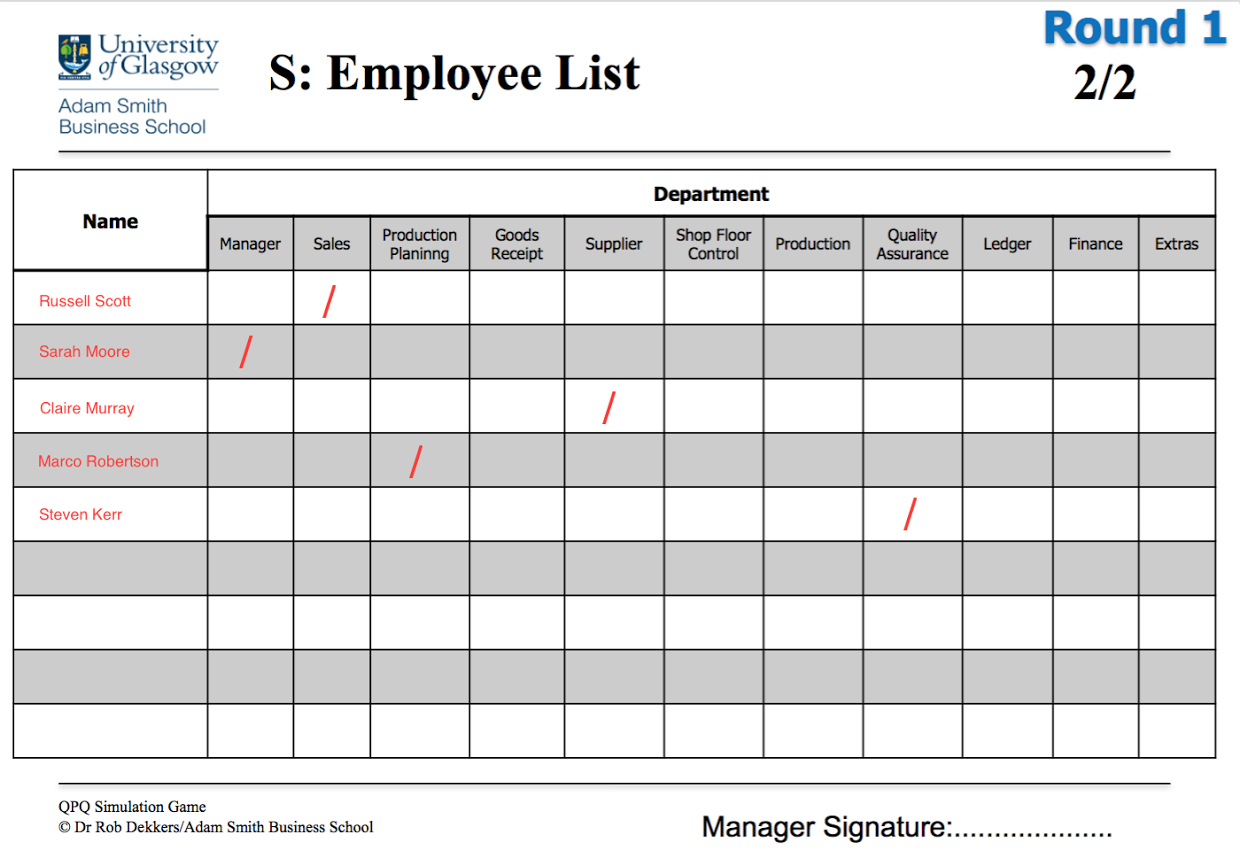
\includegraphics[width=7cm, height=4cm]{figures/paperFormS}} 
\caption{Form S}
\label{fig:FormS}
\end{figure}

\subsubsection{Form T}
\begin{figure}[!h]
\centering
\subfloat[]{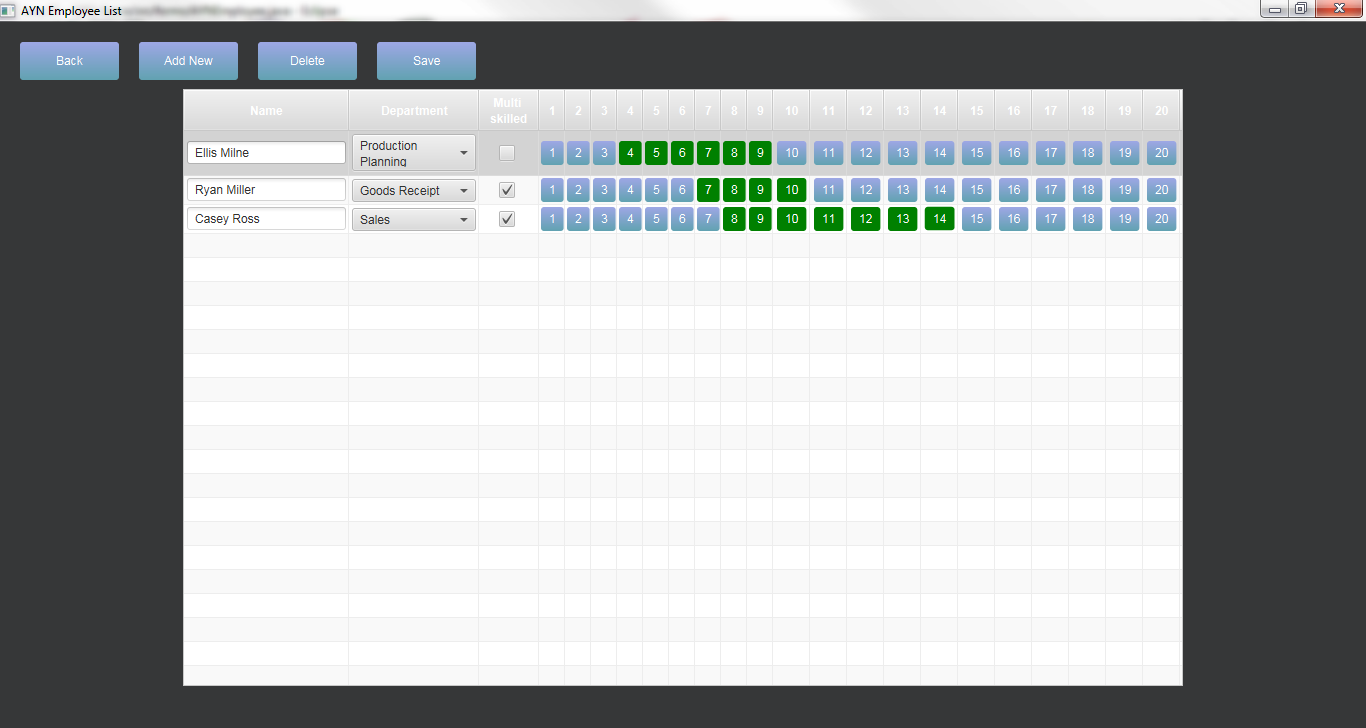
\includegraphics[width=7cm, height=4cm]{figures/AYNForm}} 
\subfloat[]{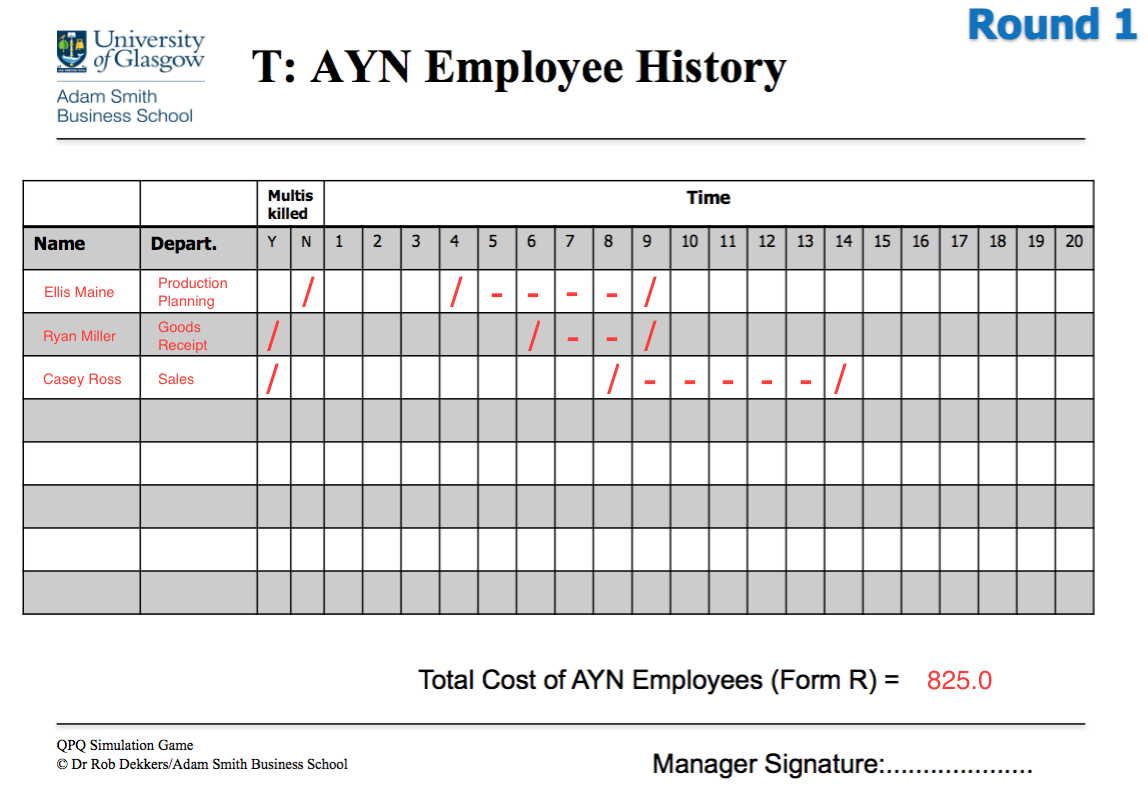
\includegraphics[width=7cm, height=4cm]{figures/AYNPaperForm}}
\caption{Form T}
\label{fig:FormT}
\end{figure}

Enter data correctly for every AYN employee. New AYN employees may be added by clicking "Add New" Button and existing AYN employees may be deleted by selecting the the employee then clicking the "Delete" button. The time of which an AYN employee worked may be input by selecting the start minute and end minute of the AYN employee on the timeline. Data will save on clicking "Back". An example is given above.

\bibliographystyle{plain}
\bibliography{dissertation}
\end{document}
